
We implemented kcores method
and tested other algorithms that are already implemented in the system with unit tests and other datasets from SNAP.

Figures below give the degree distribution and pagerank result of two dataset from SNAP. We can find that the degree distribution and pagerank results are consistent with the power law as nodes or pages with higher degree or rank have a small number while nodes or pages with lower degree or rank have a large number.
You can also find the detailed results in the output folder, which contains csv files for the results of belief propagation, connected components, node degrees, degree distribution, eigen values, k-core connected components, pagerank results, radius, etc. 


\begin{figure}[H]
\begin{center}
\begin{tabular}{cc}
     % uncomment the next lines, and give the right ps files
     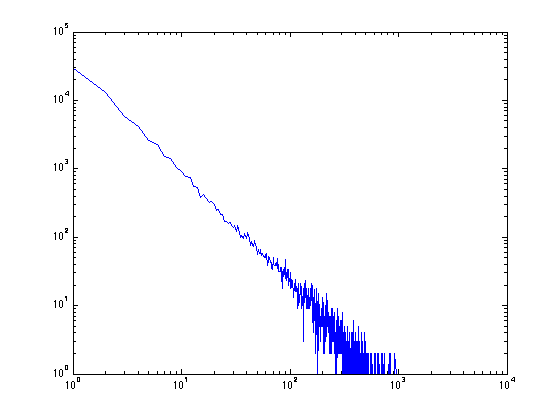
\includegraphics[width=0.3\textwidth]{FIG/soc-degreedist.png} &
     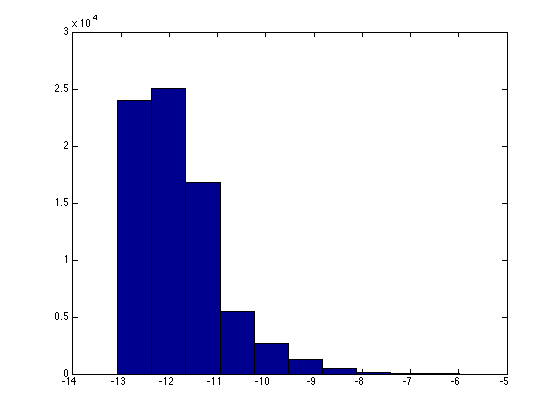
\includegraphics[width=0.3\textwidth]{FIG/soc-pagerank.png} \\
\end{tabular}
\caption{Degree Distribution(a) and PageRank(b) for Dataset SOC-Epinions1}

\begin{tabular}{cc}
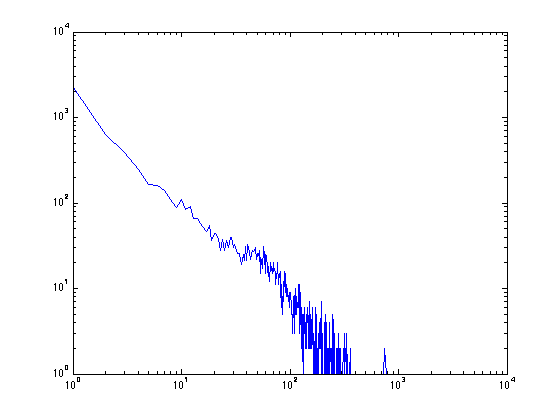
\includegraphics[width=0.3\textwidth]{FIG/wiki-degreedist.png} &
     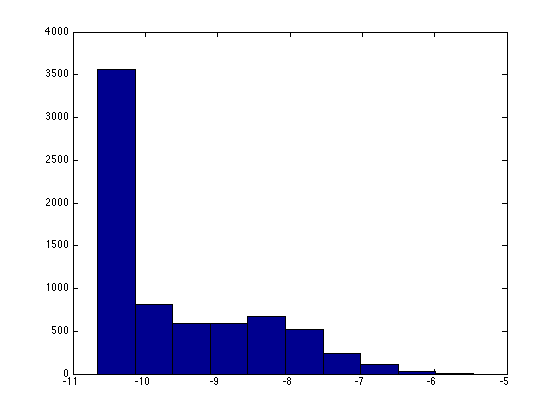
\includegraphics[width=0.3\textwidth]{FIG/wiki-pagerank.png} \\

     %\psfig{figure=FIG/plot.ps,width=2in} \\
     % \psfig{figure=FIG/data.ps,width=2in} &
     % \psfig{figure=FIG/plot.ps,width=2in} \\
    (a) & (b)
\end{tabular}
\caption{Degree Distribution(a) and PageRank(b) for Dataset wiki-Vote}

\end{center}
\end{figure}

The figures below also include the degree distribution, connected components, k=5 cores algorithm results on the 5 unit tests.
As the unit tests are small, there is no nodes in the tests that satisfy k=5 cores, so the output result for these 5 
unit tests are empty. 
However, you can find the node id, component id pairs in the stdout output from console or in the kcorecomponent.csv file, which shows that the k-core
algorithm works as it claims to find correct coreness subgraphs.

\begin{figure}[H]
\begin{center}
\begin{tabular}{cc}
     % uncomment the next lines, and give the right ps files
     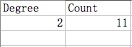
\includegraphics[width=0.3\textwidth]{FIG/1dd.jpg} &
     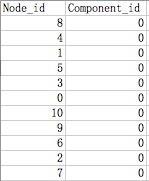
\includegraphics[width=0.3\textwidth]{FIG/1cc.jpg} \\
\end{tabular}
\caption{Degree Distribution(a), connected components(b) for Dataset1}
\end{center}
\end{figure}

\begin{figure}[H]
\begin{center}
\begin{tabular}{cc}
     % uncomment the next lines, and give the right ps files
     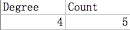
\includegraphics[width=0.3\textwidth]{FIG/2dd.jpg} &
     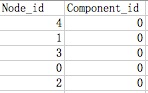
\includegraphics[width=0.3\textwidth]{FIG/2cc.jpg} \\
\end{tabular}
\caption{Degree Distribution(a), connected components(b) for Dataset2}
\end{center}
\end{figure}


\begin{figure}[H]
\begin{center}
\begin{tabular}{cc}
     % uncomment the next lines, and give the right ps files
     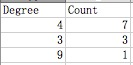
\includegraphics[width=0.3\textwidth]{FIG/3dd.jpg} &
     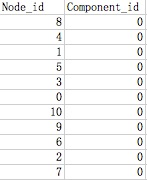
\includegraphics[width=0.3\textwidth]{FIG/3cc.jpg} \\
\end{tabular}
\caption{Degree Distribution(a), connected components(b) for Dataset3}
\end{center}
\end{figure}

\begin{figure}[H]
\begin{center}
\begin{tabular}{cc}
     % uncomment the next lines, and give the right ps files
     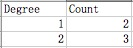
\includegraphics[width=0.3\textwidth]{FIG/4dd.jpg} &
     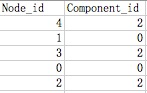
\includegraphics[width=0.3\textwidth]{FIG/4cc.jpg} \\
\end{tabular}
\caption{Degree Distribution(a), connected components(b) for Dataset4}
\end{center}
\end{figure}

\begin{figure}[H]
\begin{center}
\begin{tabular}{cc}
     % uncomment the next lines, and give the right ps files
     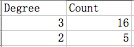
\includegraphics[width=0.3\textwidth]{FIG/5dd.jpg} &
     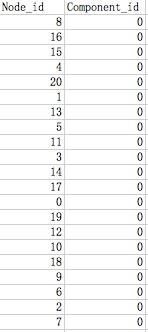
\includegraphics[width=0.3\textwidth]{FIG/5cc.jpg} \\
\end{tabular}
\caption{Degree Distribution(a) connected components(b) for Dataset5}
\end{center}
\end{figure}


We build index for algorithms Degree Distribution, K-core, Pagerank, Connected Components, All Radius, Eigen Value Computation on ten datasets:as-skitter.ungraph-75000, ca-AstroPh, cit-HepPh, cit-HepTh, com-amazon.ungraph-75000, com-dblp.ungraph-75000, email-Enron.ungraph, email-EuAll,p2p-Gnutella31, soc-Slashdot0811-75000.

We first conducted some simple tests to make sure that creating index can lead to performance improvement.
For example, 
Degree Distribution:(no index on node degree), run time is 147.476911545
Degree Distribution:(index on node degree (in degree, out degree)), run time is 346.571922302
From the experiment, create index does consume system resources and it will make performance worse in general if we
created index and used it only once.
However, 
Degree Distribution:(no index on node degree)(run 10 times), run time is 2091.14193916,
Degree Distribution:(index on node degree (in degree, out degree))(run 10 times, 1 time create index), run time is 1351.35889053.
From the experiment, create index will improve performance in general if we created index and used it later a lot.
Also, for a certain algorithm, create index for some tables like GMNODES are expensive, but if re run all the algorithms,or use the algorithm multiple times, then the cost of creating index on tables like GMNODES will be worth the effort.

This is the general intuitive for us to choose on which table and which column to create index and avoid some unnecessay tests.

We compared building index for different tables on different columns for each algorithm and get the following figures below. 

\begin{figure}[H]
\begin{center}
\begin{tabular}{cc}
     % uncomment the next lines, and give the right ps files
     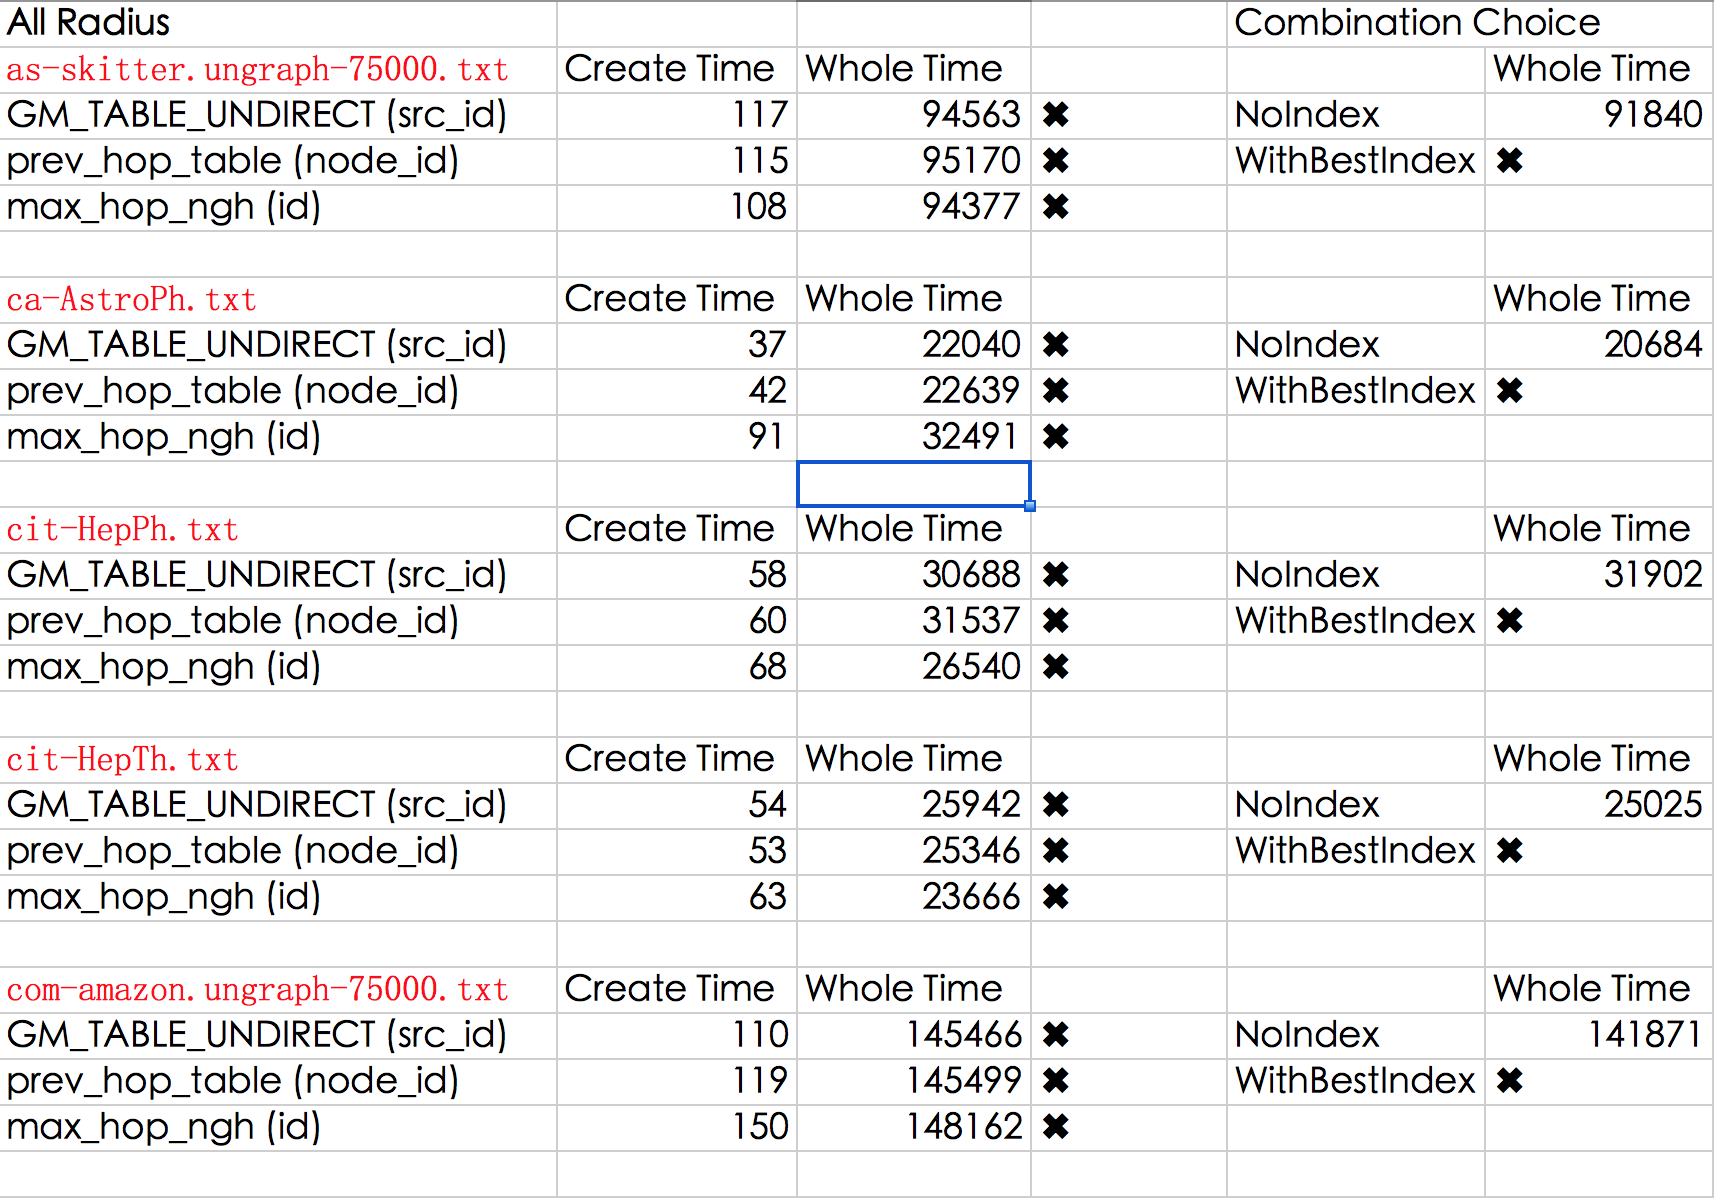
\includegraphics[width=1.0\textwidth]{FIG/AllRadius1.png} \\
     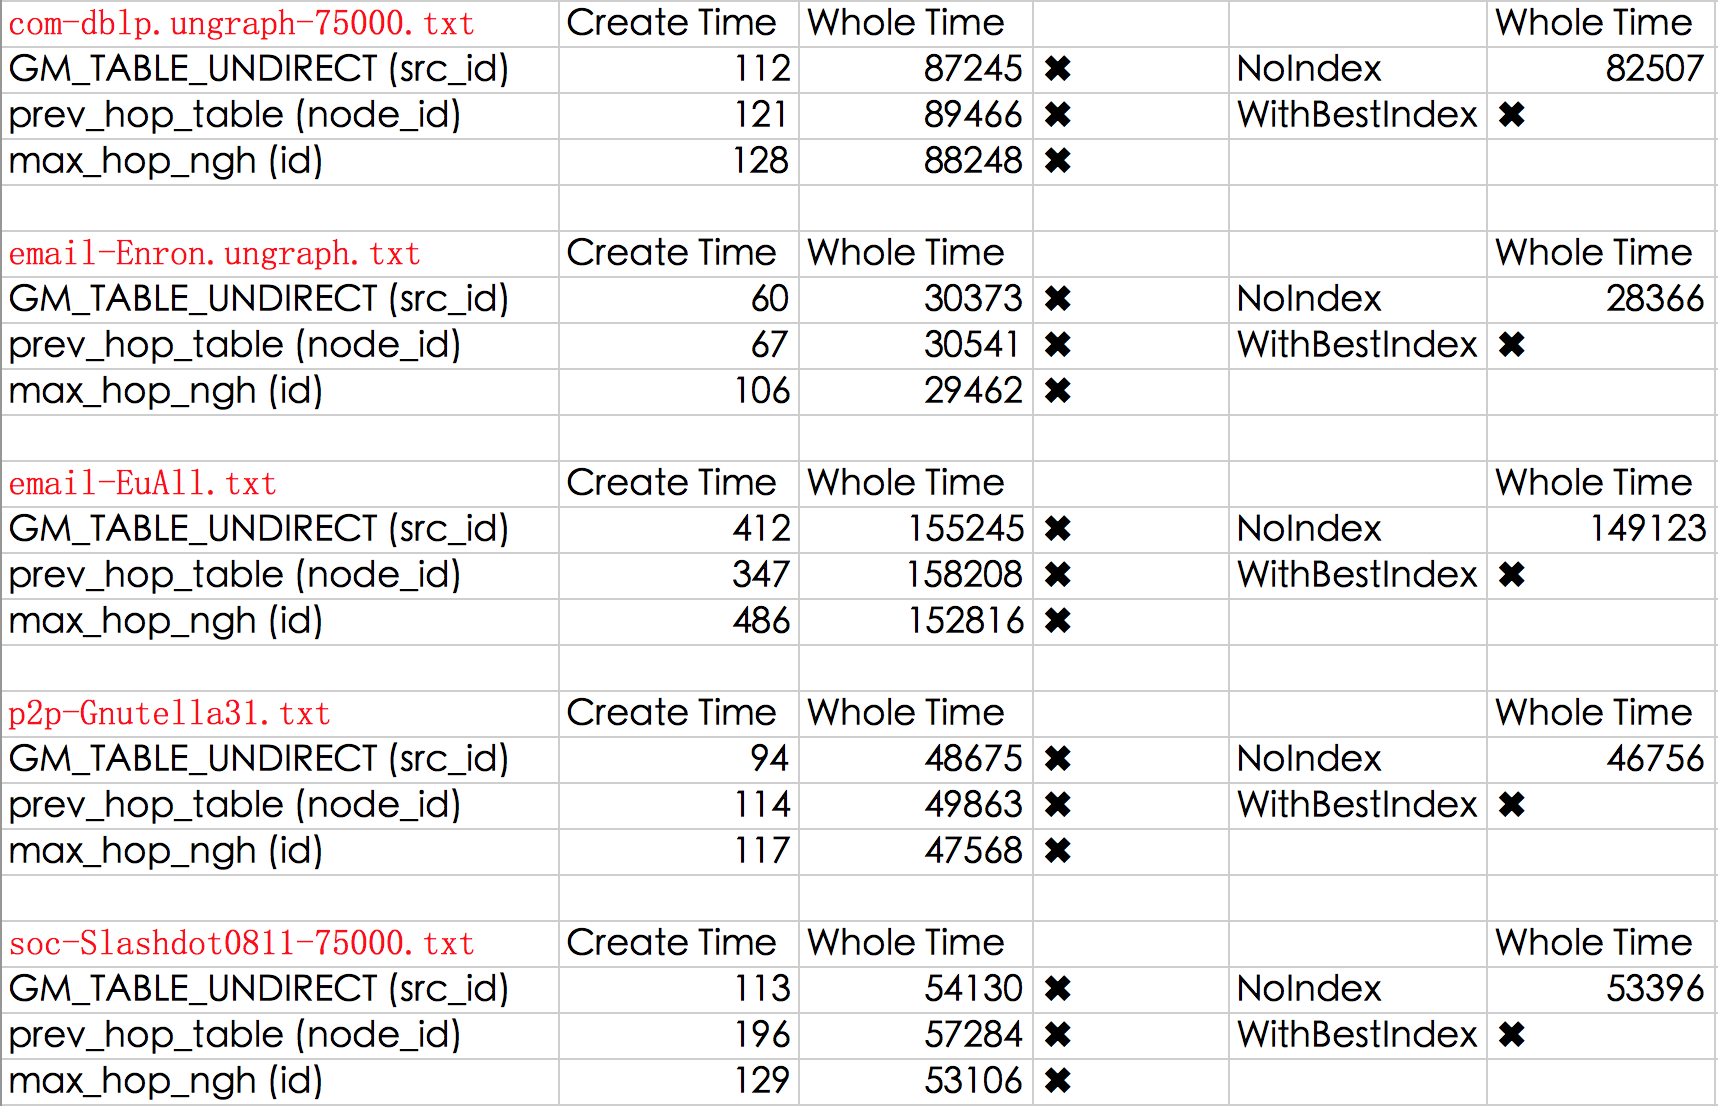
\includegraphics[width=1.0\textwidth]{FIG/AllRadius2.png} \\
\end{tabular}
\caption{Creating Index Experiments on All Radius Algorithm}
\end{center}
\end{figure}

\begin{figure}[H]
\begin{center}
\begin{tabular}{cc}
     % uncomment the next lines, and give the right ps files
     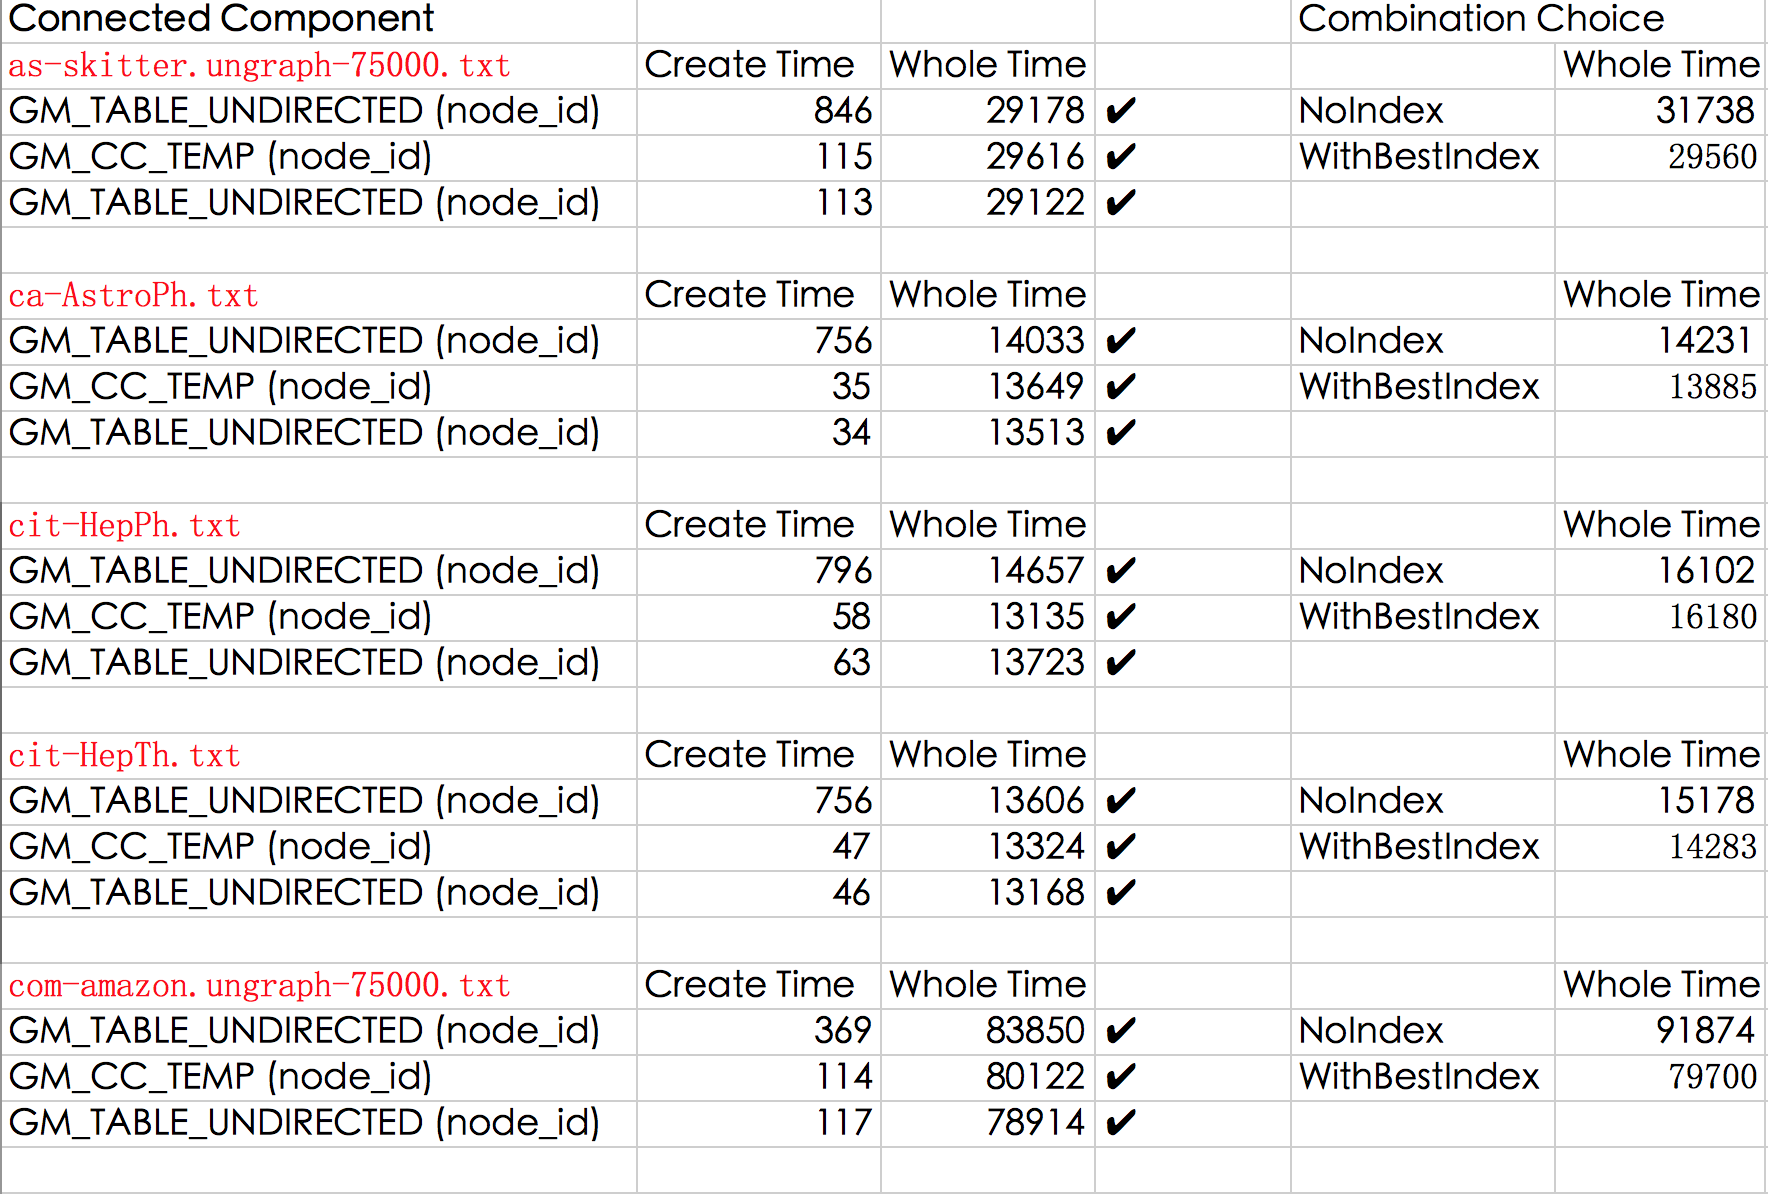
\includegraphics[width=1.0\textwidth]{FIG/CC1.png} \\
     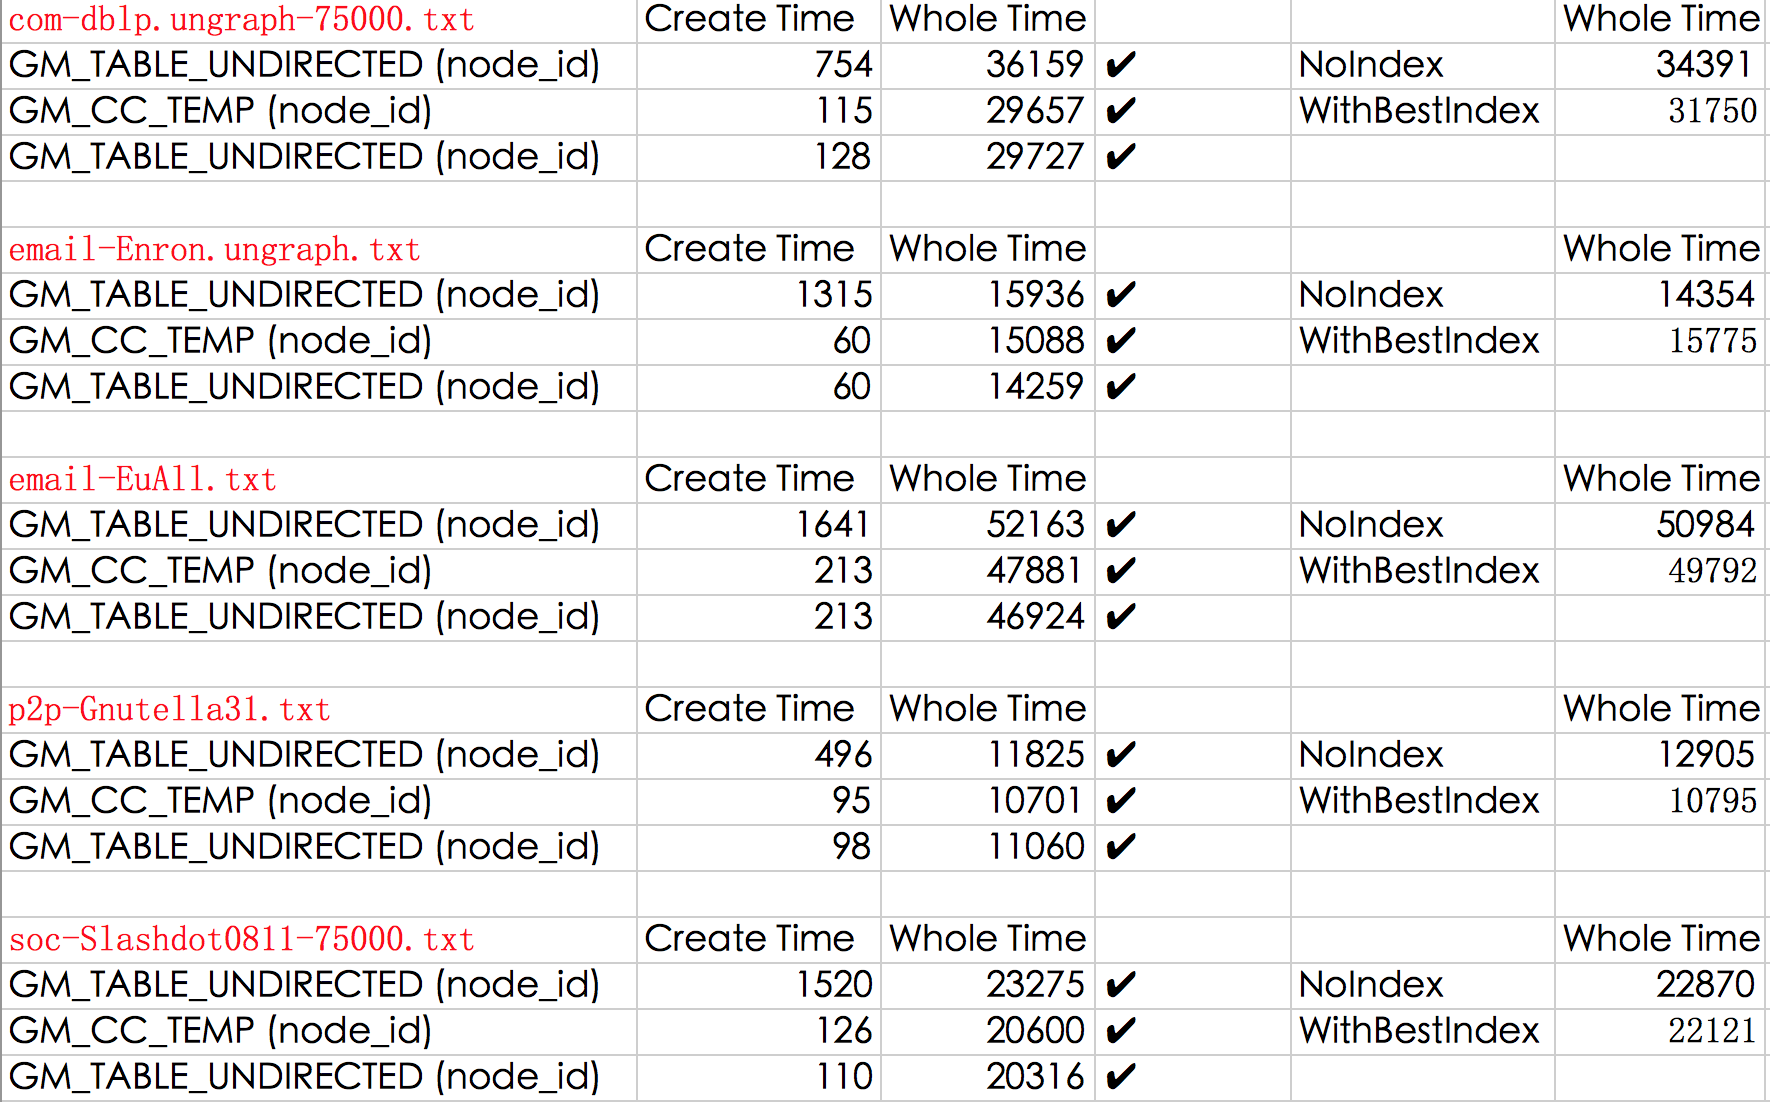
\includegraphics[width=1.0\textwidth]{FIG/CC2.png} \\
\end{tabular}
\caption{Creating Index Experiments on Connected Components Algorithm}
\end{center}
\end{figure}

\begin{figure}[H]
\begin{center}
\begin{tabular}{cc}
     % uncomment the next lines, and give the right ps files
     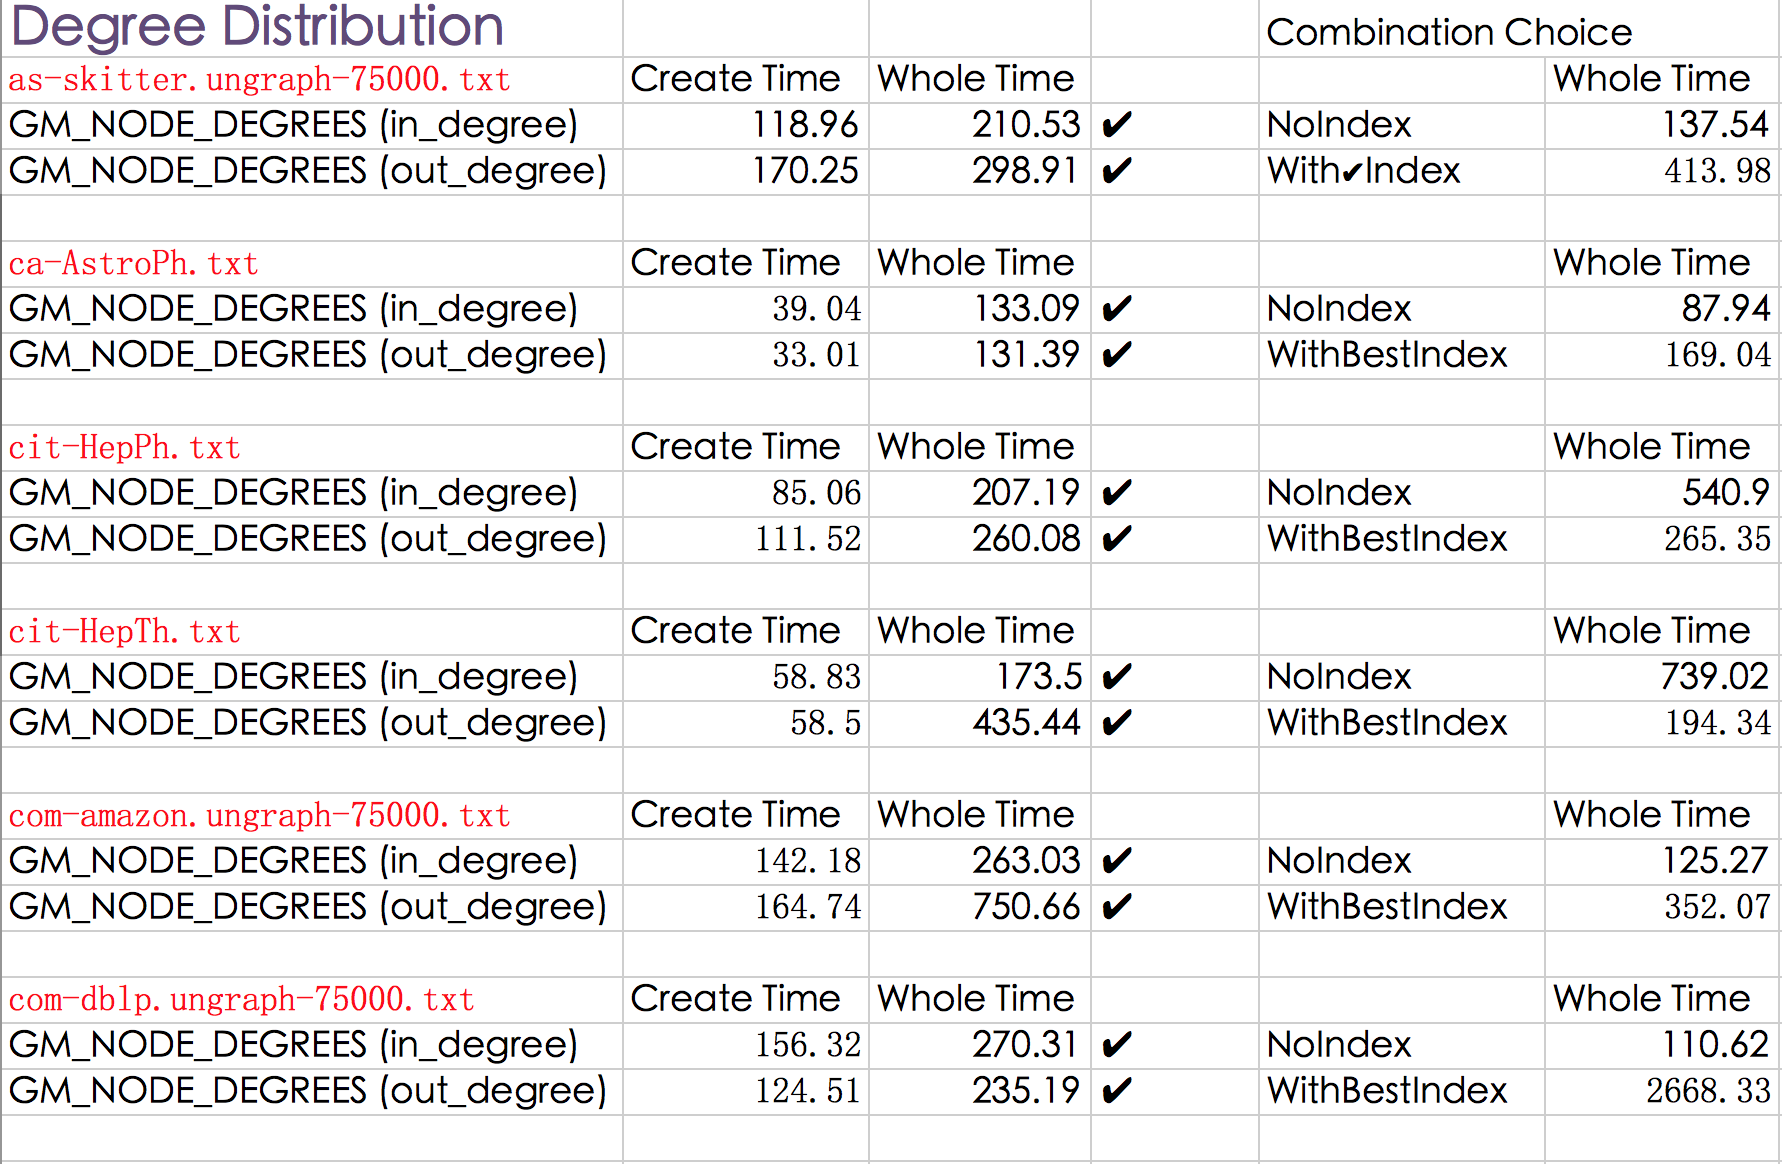
\includegraphics[width=1.0\textwidth]{FIG/DD1.png} \\
     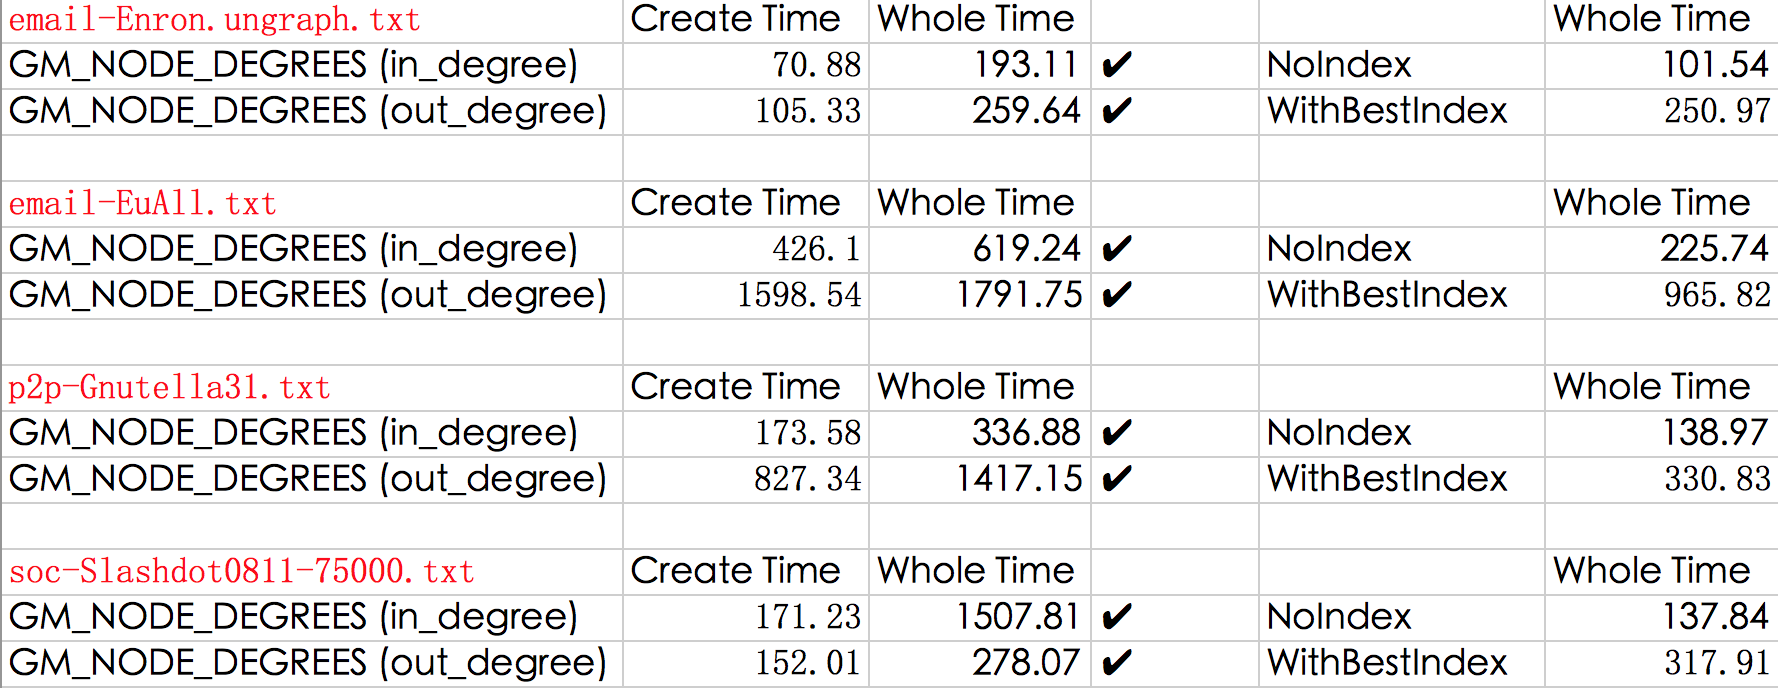
\includegraphics[width=1.0\textwidth]{FIG/DD2.png} \\
\end{tabular}
\caption{Creating Index Experiments on Degree Distribution Algorithm}
\end{center}
\end{figure}

\begin{figure}[H]
\begin{center}
\begin{tabular}{cc}
     % uncomment the next lines, and give the right ps files
     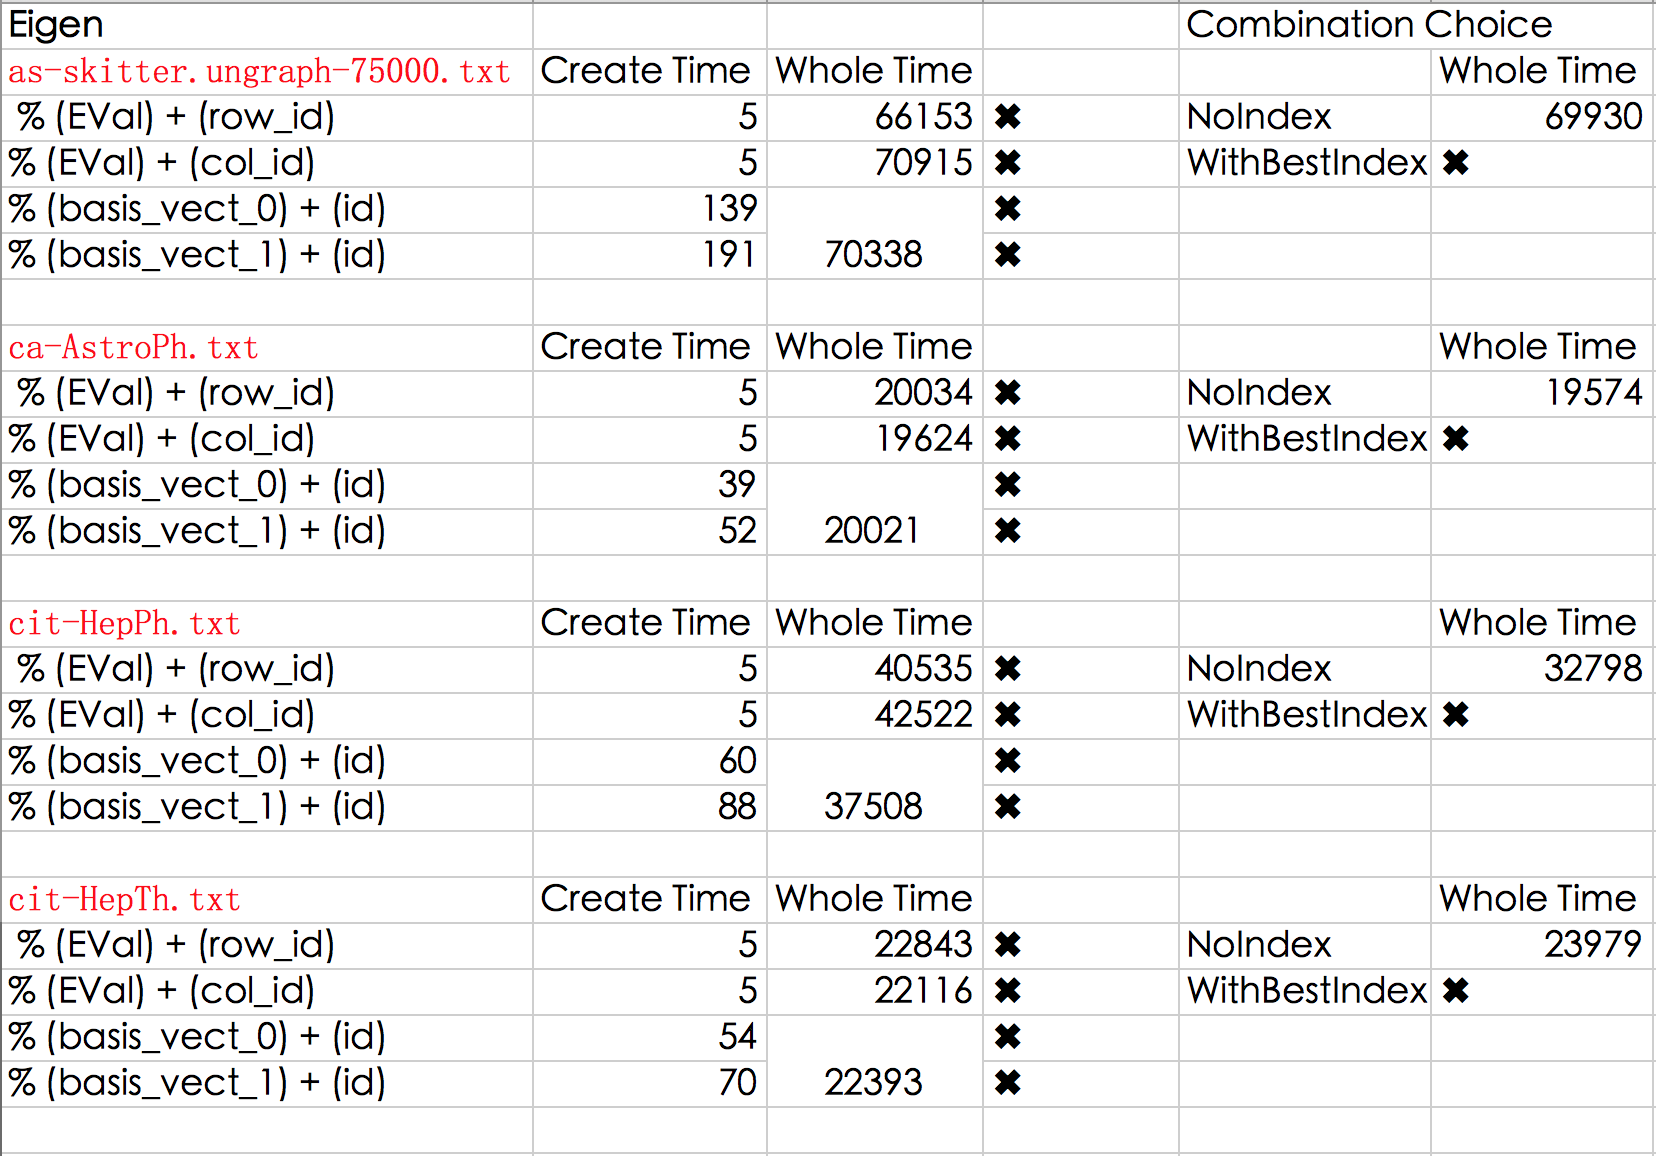
\includegraphics[width=1.0\textwidth]{FIG/Eigen1.png} \\
     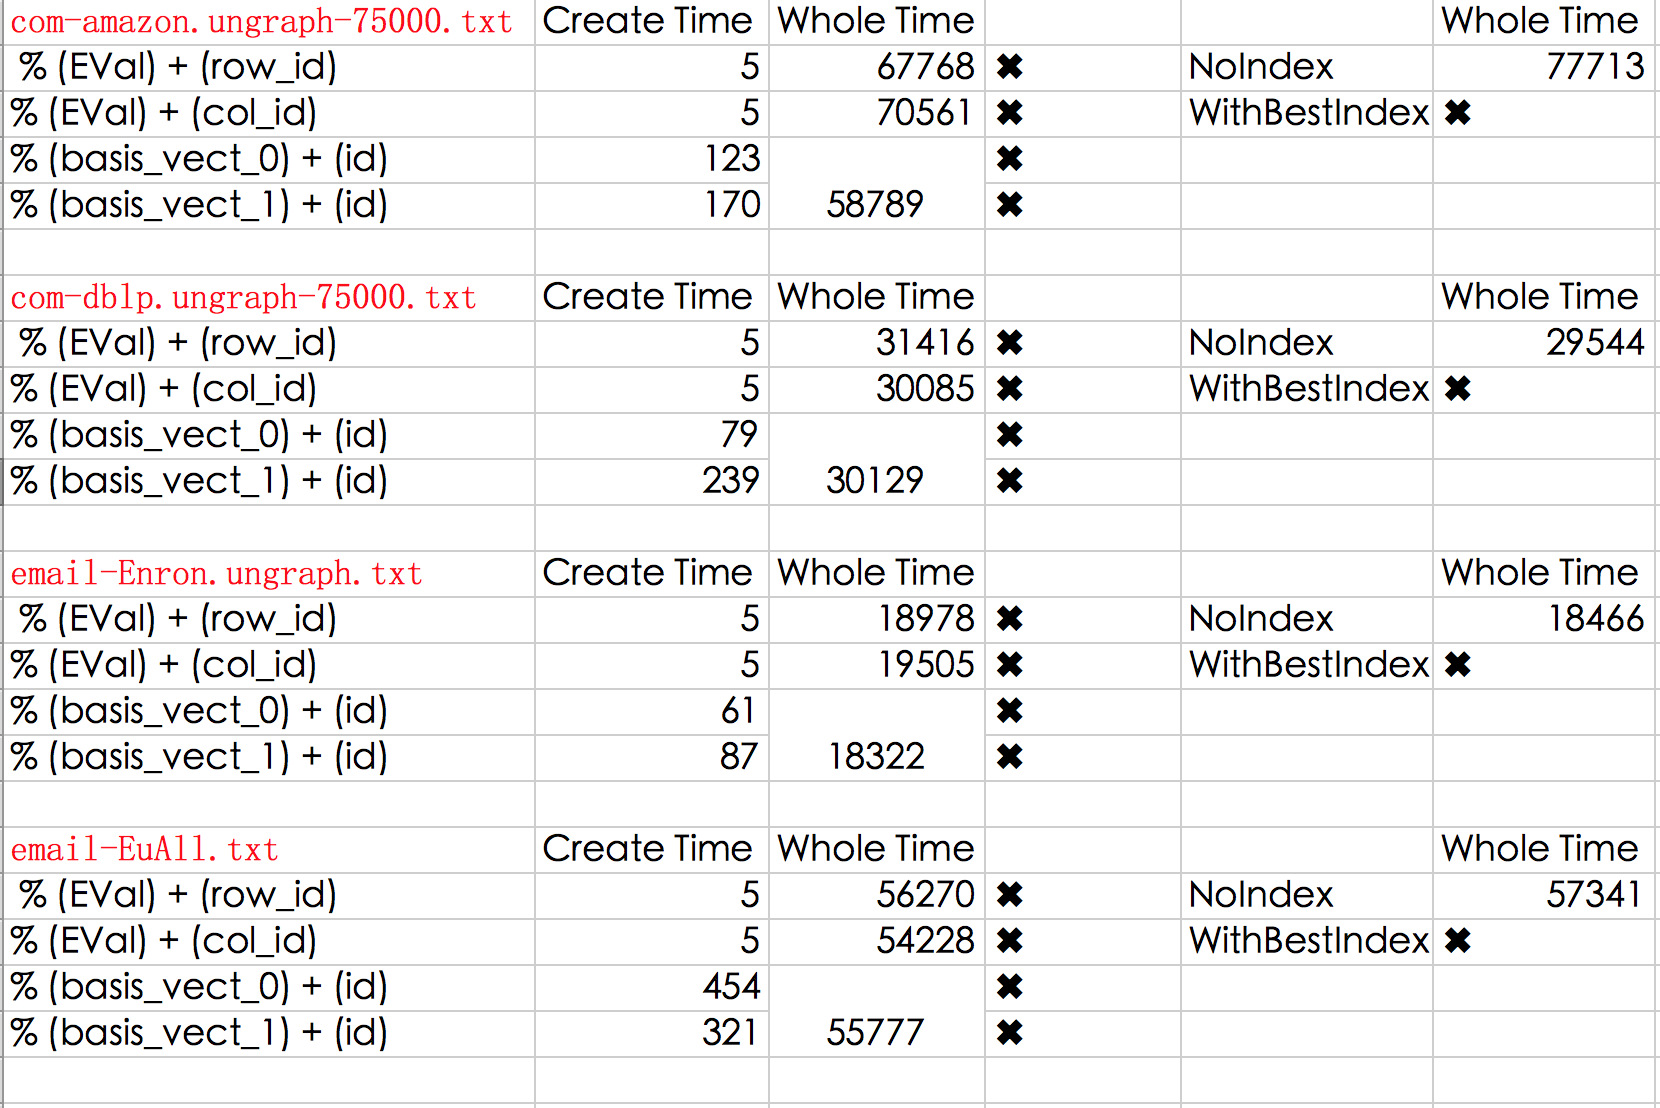
\includegraphics[width=1.0\textwidth]{FIG/Eigen2.png} \\
     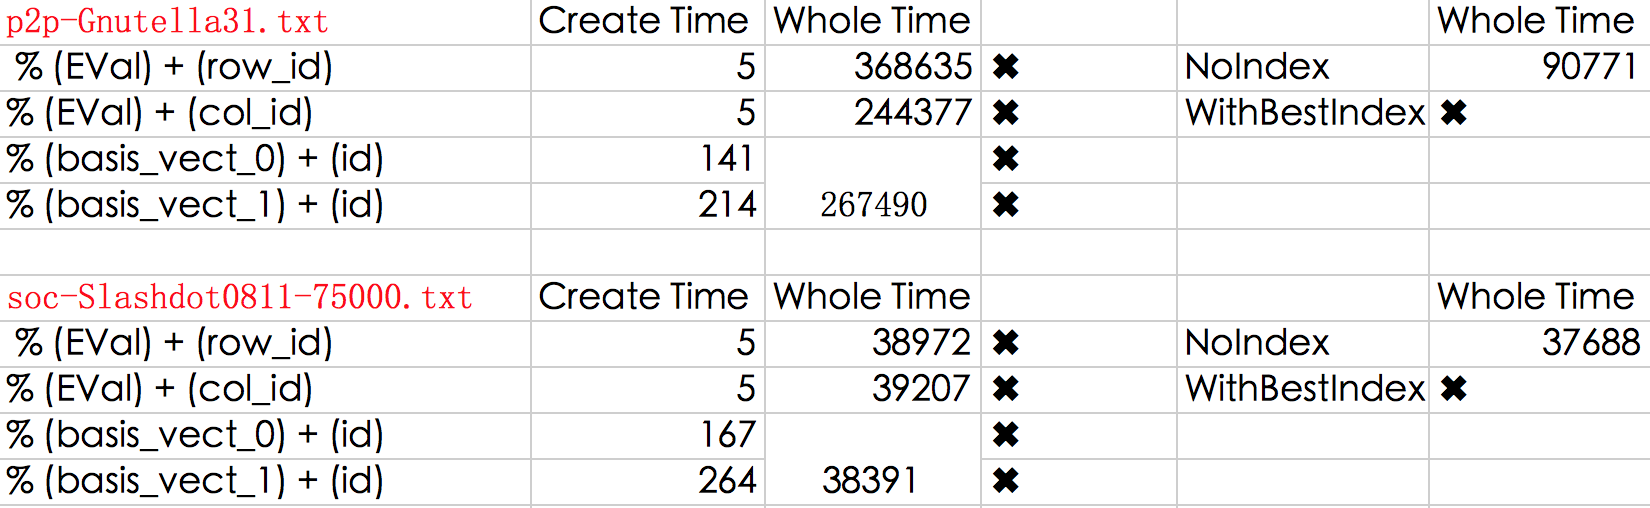
\includegraphics[width=1.0\textwidth]{FIG/Eigen3.png} \\
\end{tabular}
\caption{Creating Index Experiments on Eigen Value Computation Algorithm}
\end{center}
\end{figure}

\begin{figure}[H]
\begin{center}
\begin{tabular}{cc}
     % uncomment the next lines, and give the right ps files
     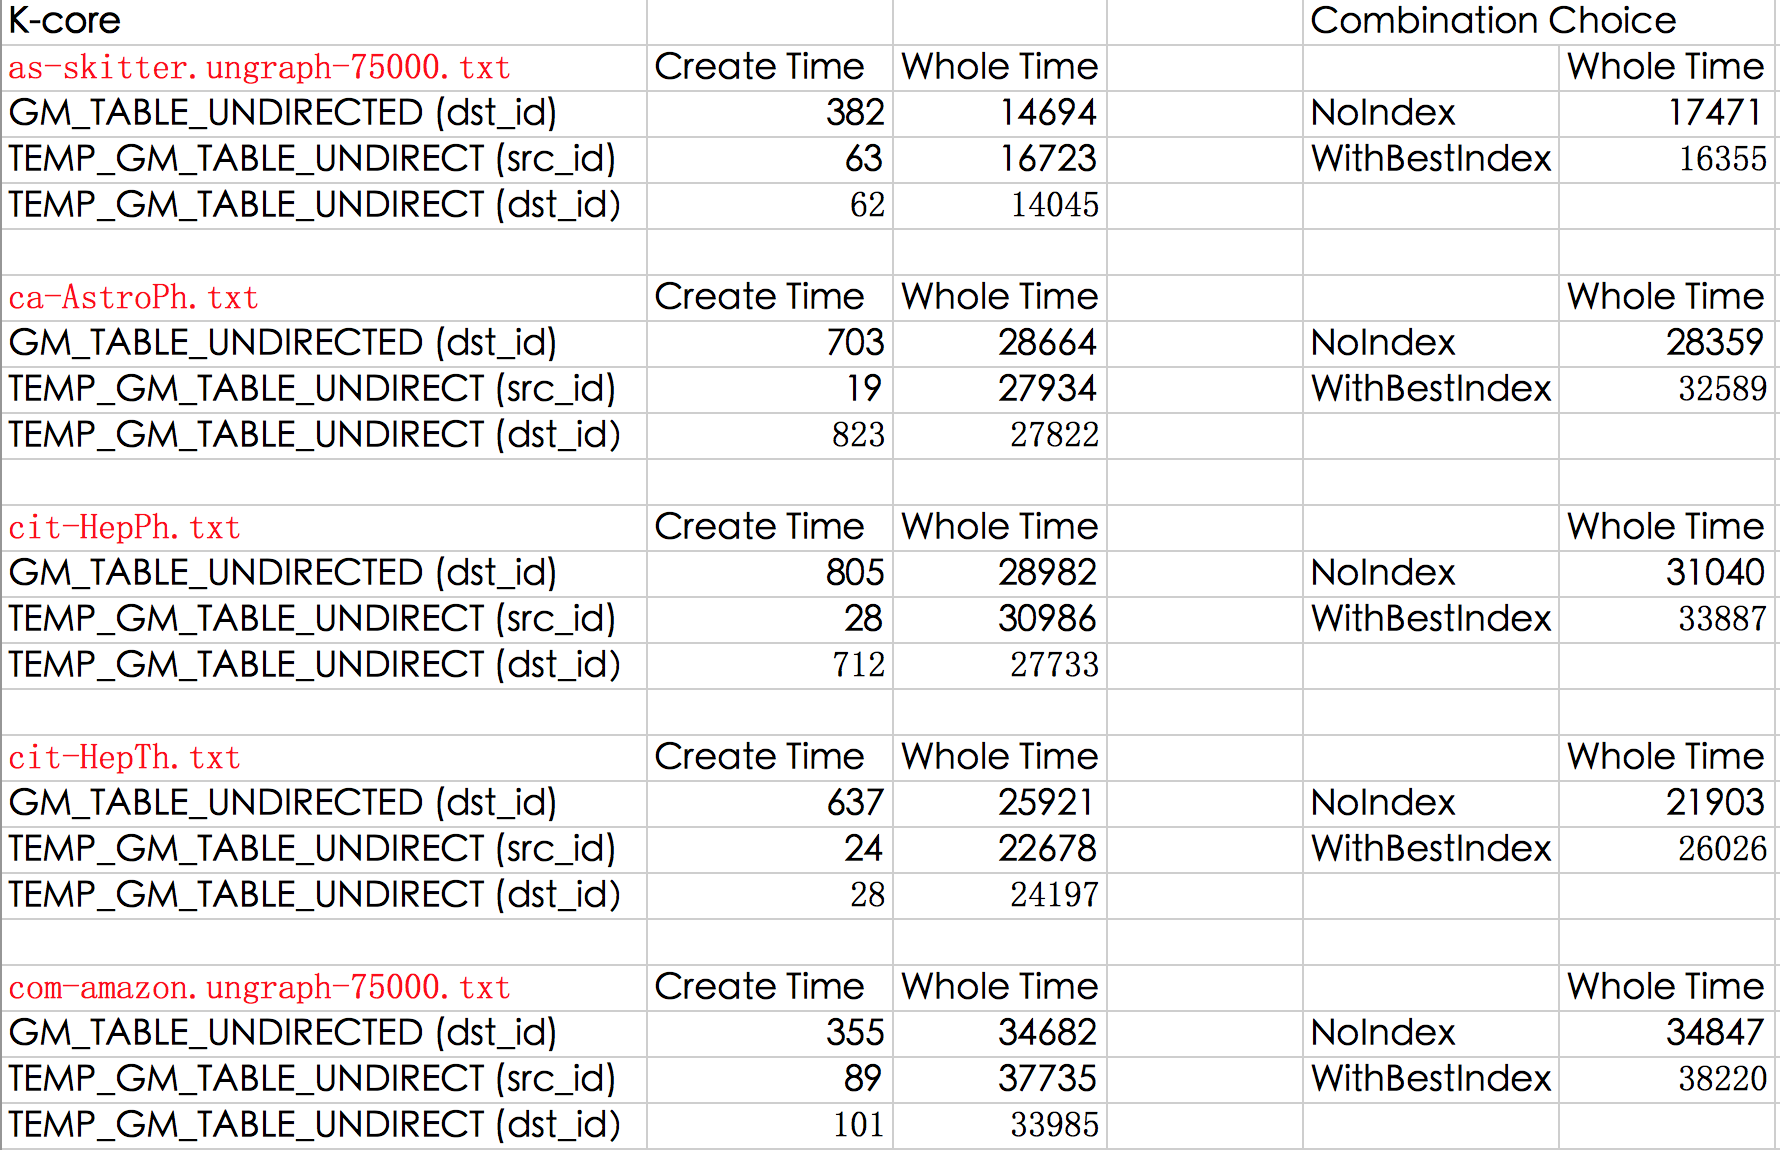
\includegraphics[width=1.0\textwidth]{FIG/KC1.png} \\
     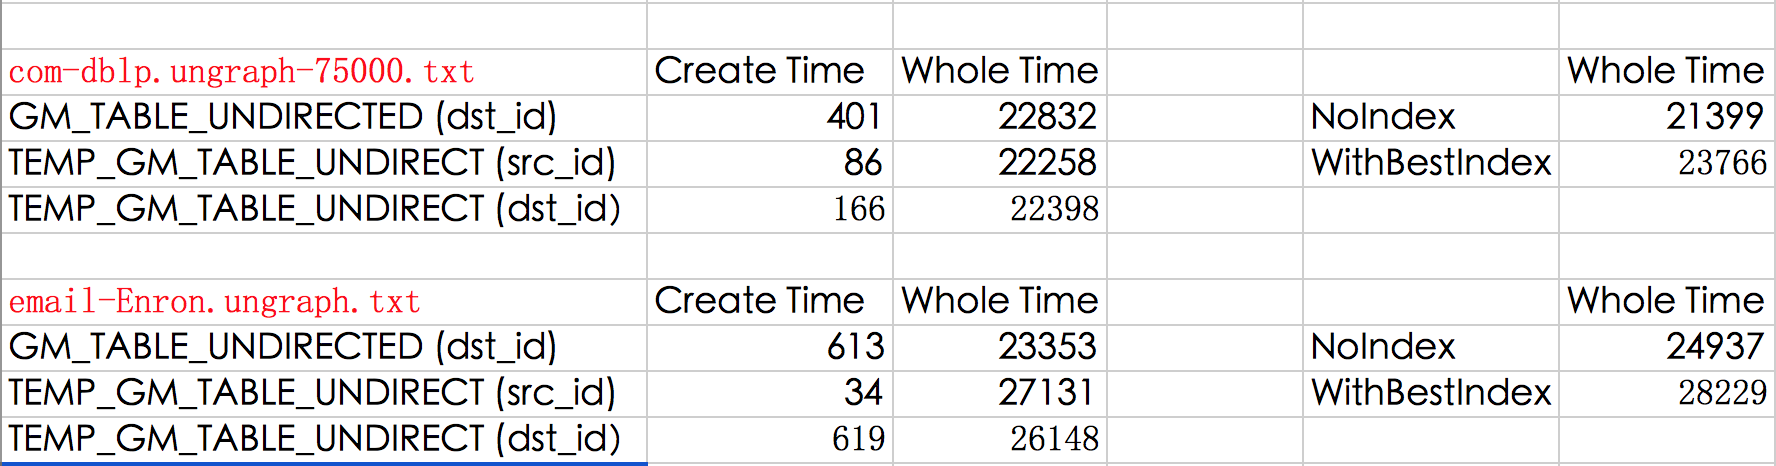
\includegraphics[width=1.0\textwidth]{FIG/KC2.png} \\
\end{tabular}
\caption{Creating Index Experiments on K-core Algorithm}
\end{center}
\end{figure}

\begin{figure}[H]
\begin{center}
\begin{tabular}{cc}
     % uncomment the next lines, and give the right ps files
     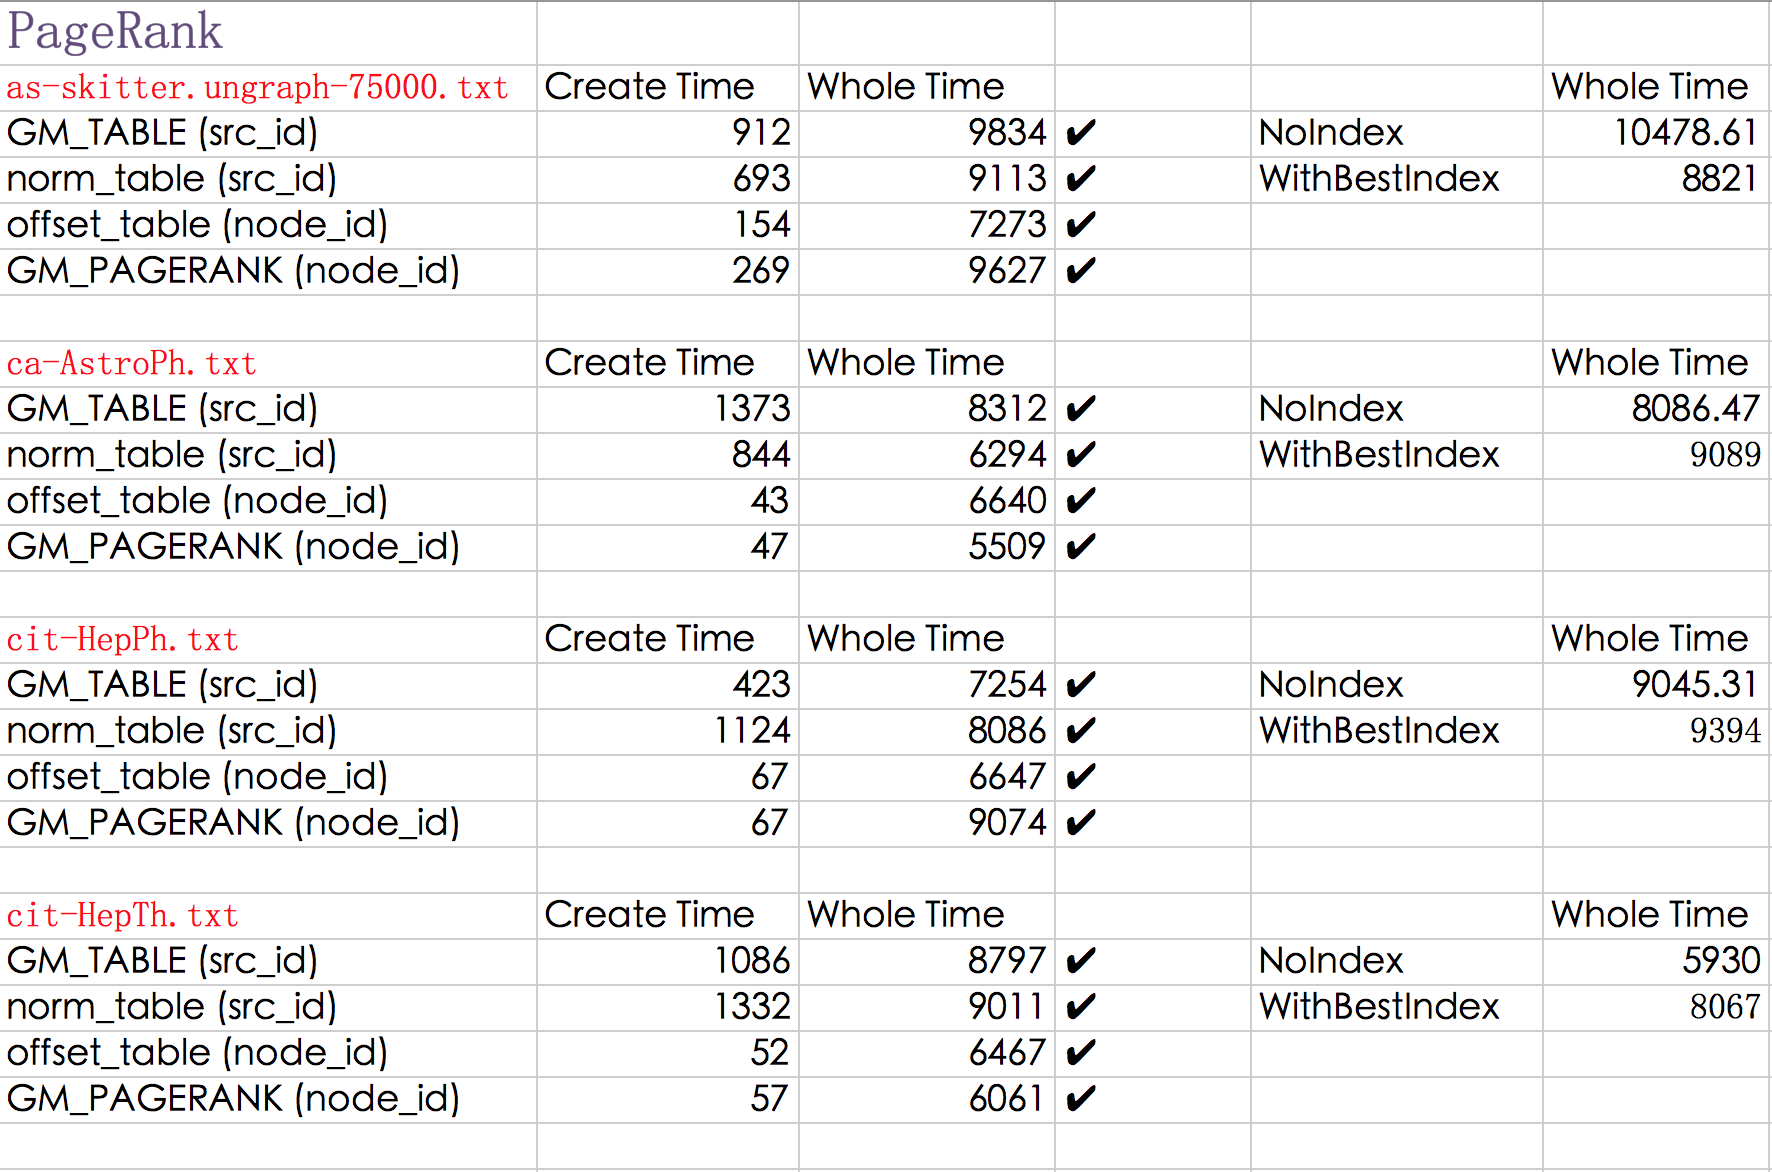
\includegraphics[width=1.0\textwidth]{FIG/PR1.png} \\
     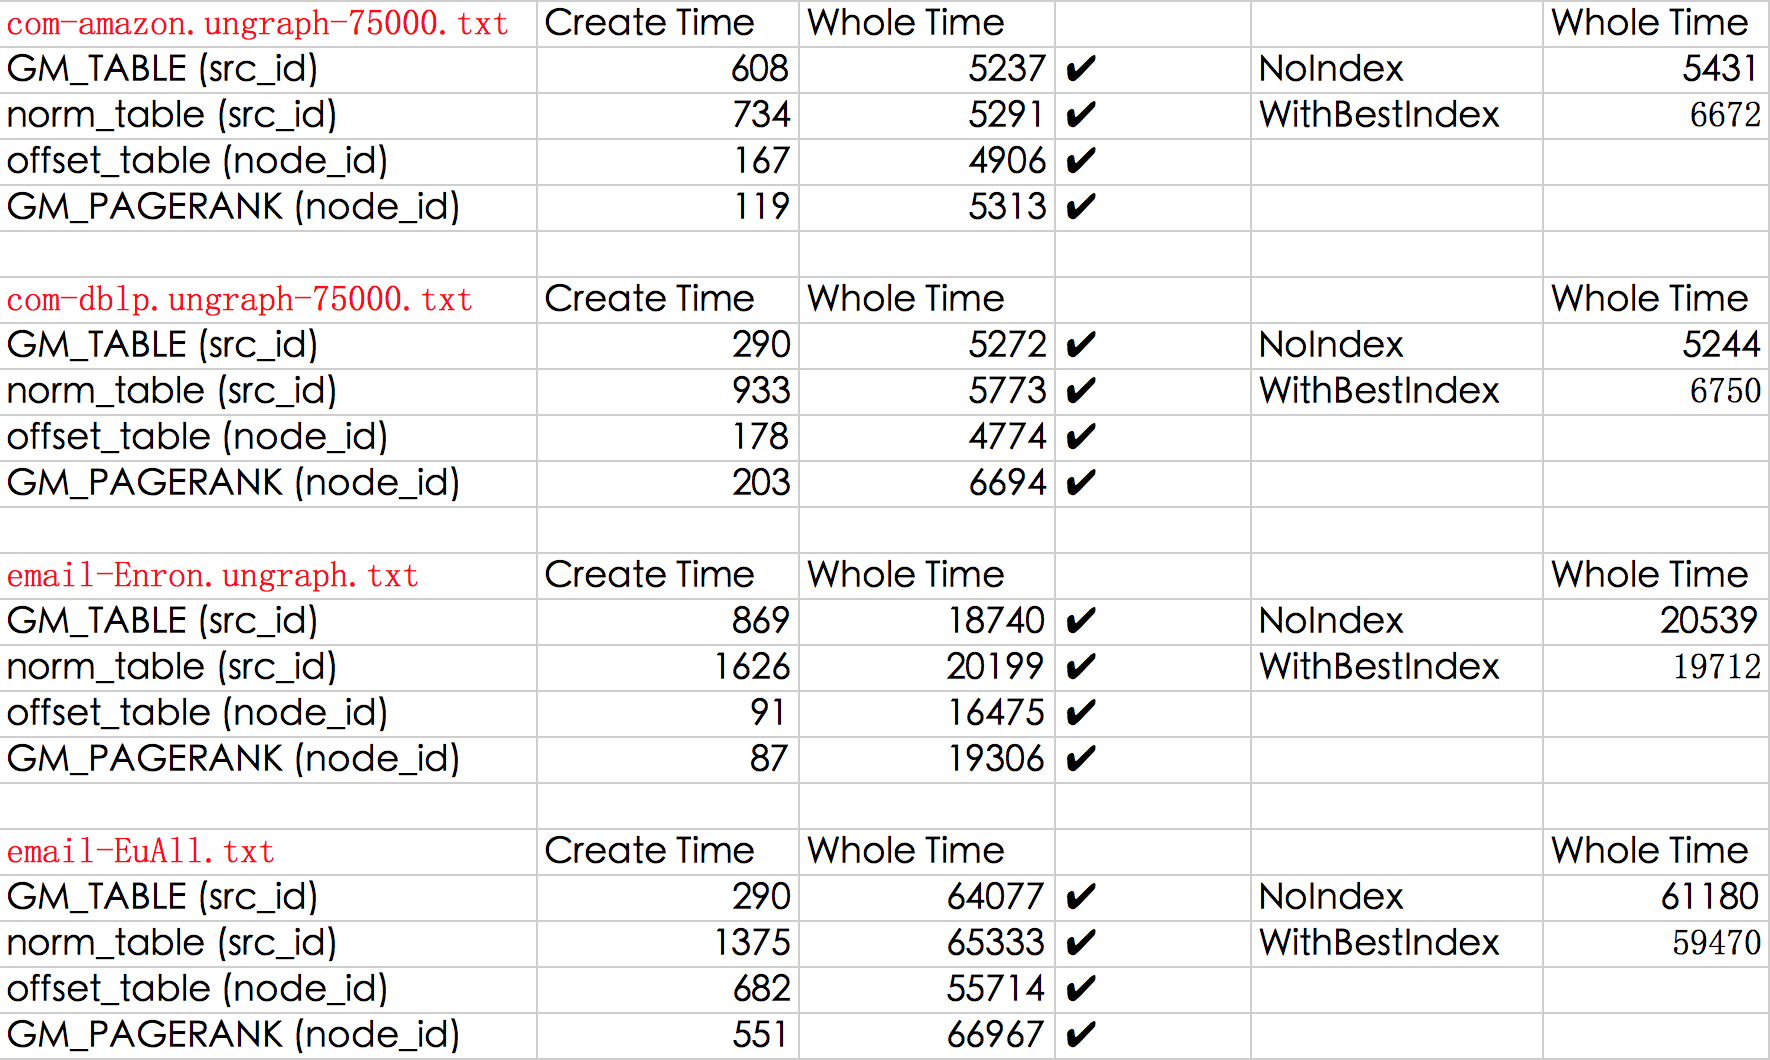
\includegraphics[width=1.0\textwidth]{FIG/PR2.png} \\
\end{tabular}
\caption{Creating Index Experiments on PageRank Algorithm}
\end{center}
\end{figure}


The following are the results of the degree distribution and pagerank results for the ten datasets.
\begin{figure}[H]
\begin{center}
\begin{tabular}{cc}
     % uncomment the next lines, and give the right ps files
     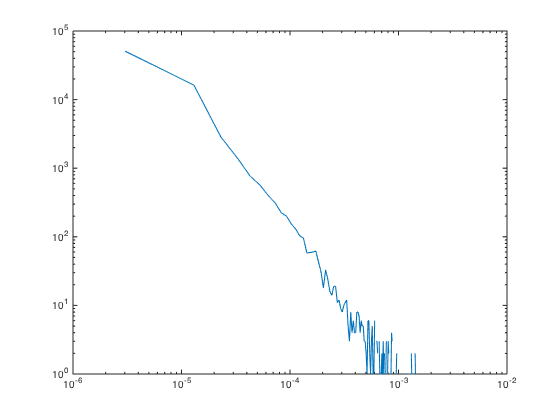
\includegraphics[width=0.3\textwidth]{FIG/1pagerank.png} &
     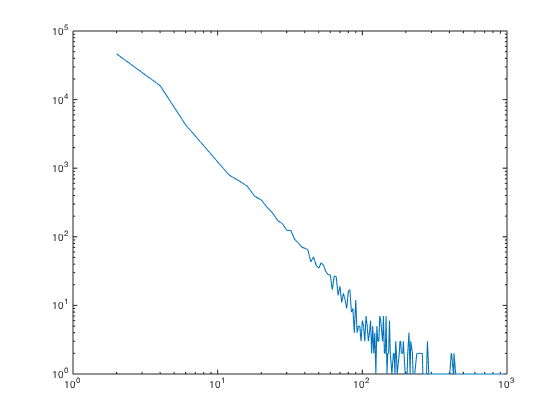
\includegraphics[width=0.3\textwidth]{FIG/1degreedist.png} \\
\end{tabular}
\caption{Result on PageRank Algorithm and Degree Distribution}
\end{center}
\end{figure}

\begin{figure}[H]
\begin{center}
\begin{tabular}{cc}
     % uncomment the next lines, and give the right ps files
     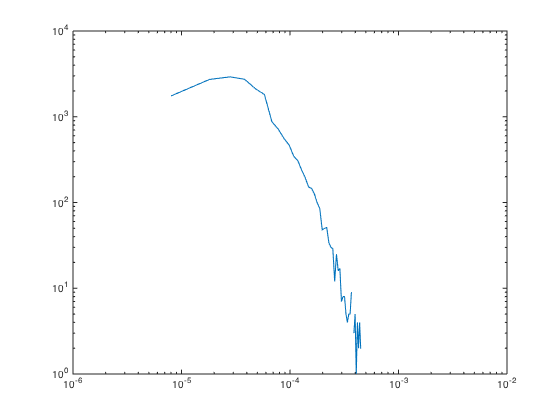
\includegraphics[width=0.3\textwidth]{FIG/2pagerank.png} &
     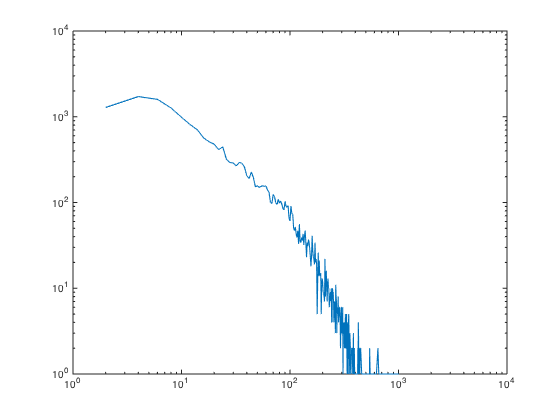
\includegraphics[width=0.3\textwidth]{FIG/2degreedist.png} \\
\end{tabular}
\caption{Result on PageRank Algorithm and Degree Distribution}
\end{center}
\end{figure}

\begin{figure}[H]
\begin{center}
\begin{tabular}{cc}
     % uncomment the next lines, and give the right ps files
     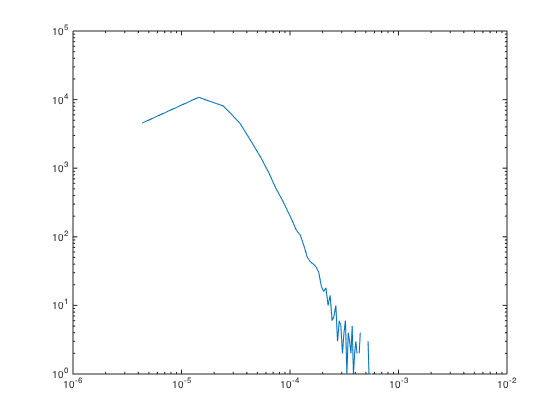
\includegraphics[width=0.3\textwidth]{FIG/3pagerank.png} &
     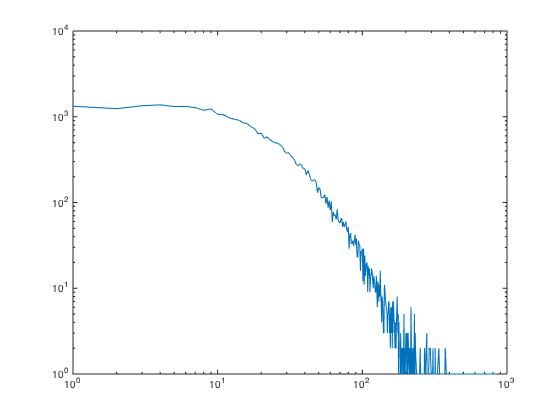
\includegraphics[width=0.3\textwidth]{FIG/3degreedist.png} \\
\end{tabular}
\caption{Result on PageRank Algorithm and Degree Distribution}
\end{center}
\end{figure}

\begin{figure}[H]
\begin{center}
\begin{tabular}{cc}
     % uncomment the next lines, and give the right ps files
     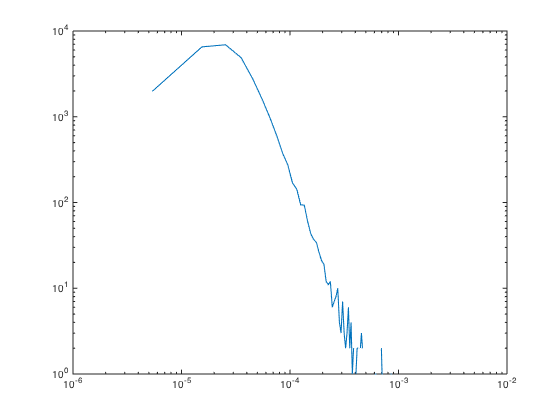
\includegraphics[width=0.3\textwidth]{FIG/4pagerank.png} &
     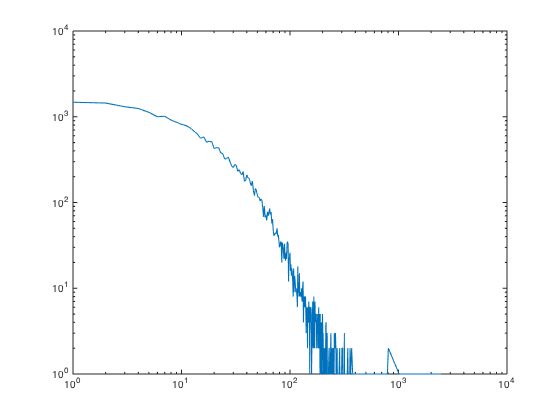
\includegraphics[width=0.3\textwidth]{FIG/4degreedist.png} \\
\end{tabular}
\caption{Result on PageRank Algorithm and Degree Distribution}
\end{center}
\end{figure}

\begin{figure}[H]
\begin{center}
\begin{tabular}{cc}
     % uncomment the next lines, and give the right ps files
     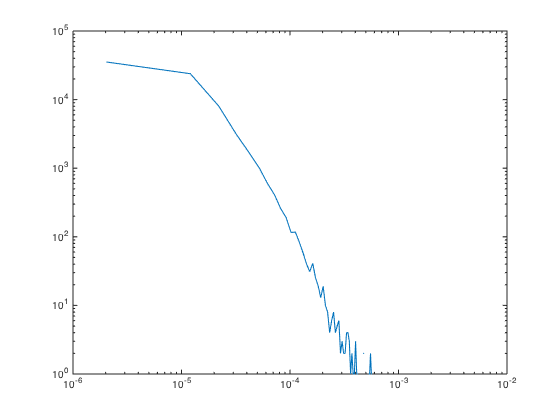
\includegraphics[width=0.3\textwidth]{FIG/5pagerank.png} &
     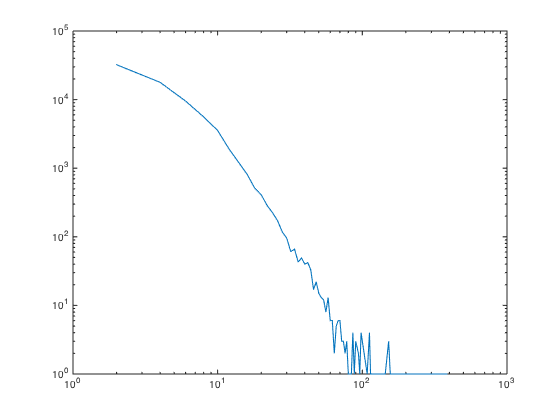
\includegraphics[width=0.3\textwidth]{FIG/5degreedist.png} \\
\end{tabular}
\caption{Result on PageRank Algorithm and Degree Distribution}
\end{center}
\end{figure}

\begin{figure}[H]
\begin{center}
\begin{tabular}{cc}
     % uncomment the next lines, and give the right ps files
     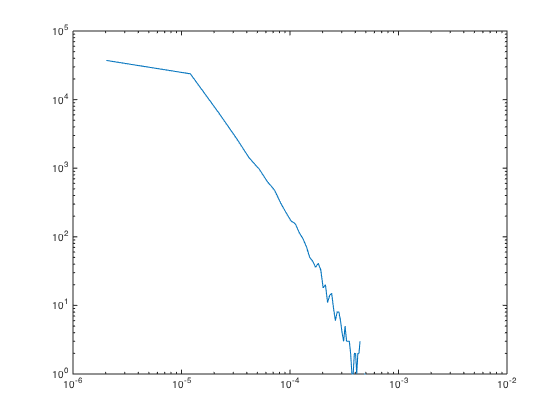
\includegraphics[width=0.3\textwidth]{FIG/6pagerank.png} &
     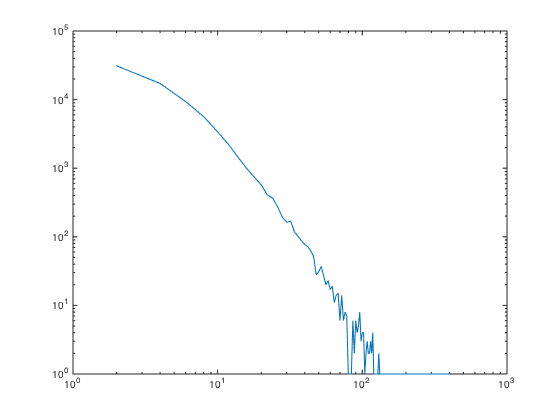
\includegraphics[width=0.3\textwidth]{FIG/6degreedist.png} \\
\end{tabular}
\caption{Result on PageRank Algorithm and Degree Distribution}
\end{center}
\end{figure}

\begin{figure}[H]
\begin{center}
\begin{tabular}{cc}
     % uncomment the next lines, and give the right ps files
     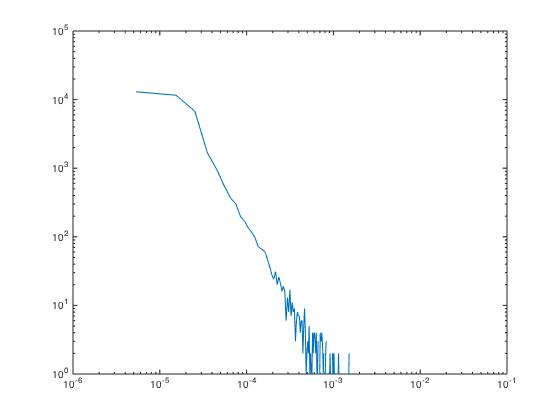
\includegraphics[width=0.3\textwidth]{FIG/7pagerank.png} &
     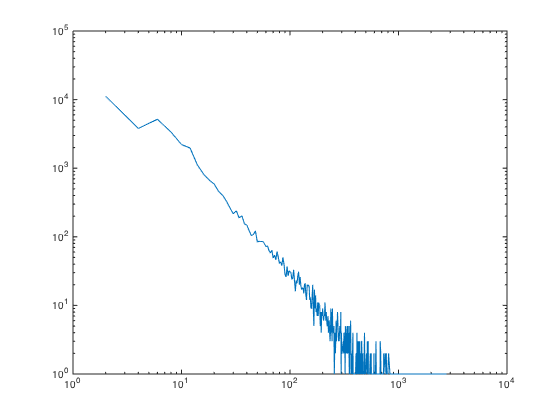
\includegraphics[width=0.3\textwidth]{FIG/7degreedist.png} \\
\end{tabular}
\caption{Result on PageRank Algorithm and Degree Distribution}
\end{center}
\end{figure}

\begin{figure}[H]
\begin{center}
\begin{tabular}{cc}
     % uncomment the next lines, and give the right ps files
     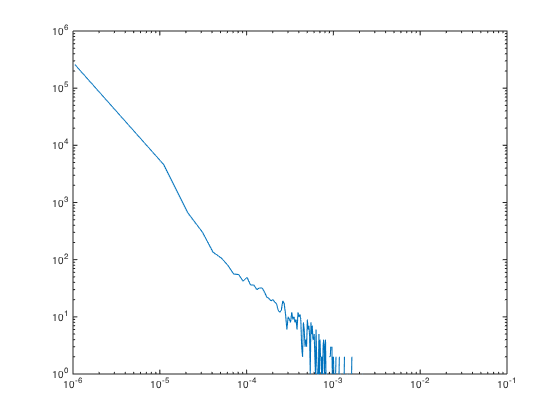
\includegraphics[width=0.3\textwidth]{FIG/8pagerank.png} &
     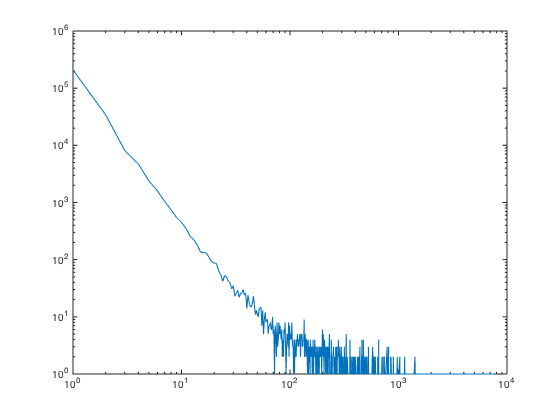
\includegraphics[width=0.3\textwidth]{FIG/8degreedist.png} \\
\end{tabular}
\caption{Result on PageRank Algorithm and Degree Distribution}
\end{center}
\end{figure}

\begin{figure}[H]
\begin{center}
\begin{tabular}{cc}
     % uncomment the next lines, and give the right ps files
     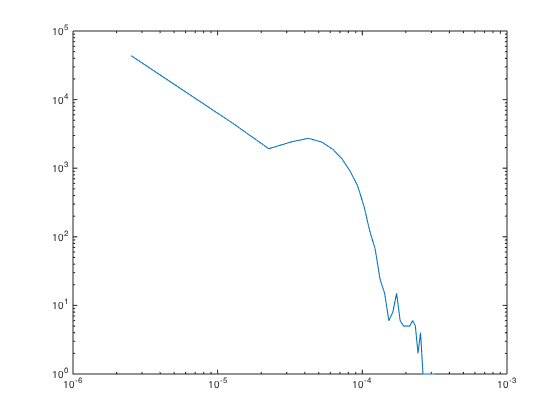
\includegraphics[width=0.3\textwidth]{FIG/9pagerank.png} &
     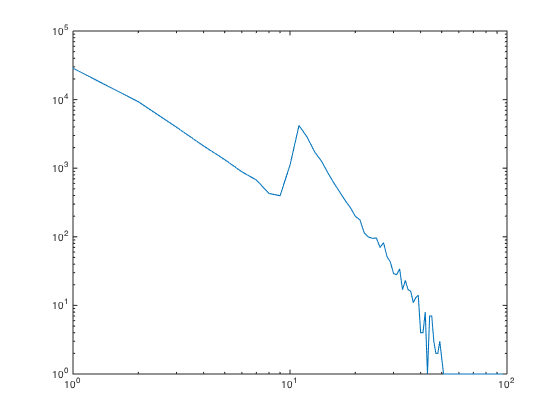
\includegraphics[width=0.3\textwidth]{FIG/9degreedist.png} \\
\end{tabular}
\caption{Result on PageRank Algorithm and Degree Distribution}
\end{center}
\end{figure}

\begin{figure}[H]
\begin{center}
\begin{tabular}{cc}
     % uncomment the next lines, and give the right ps files
     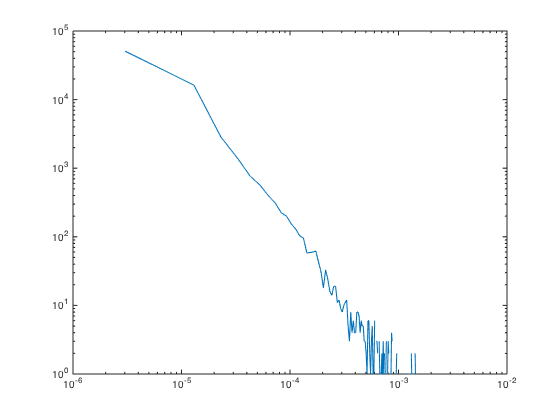
\includegraphics[width=0.3\textwidth]{FIG/1pagerank.png} &
     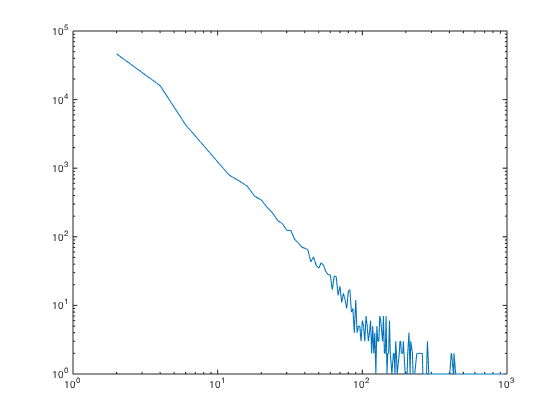
\includegraphics[width=0.3\textwidth]{FIG/1degreedist.png} \\
\end{tabular}
\caption{Result on PageRank Algorithm and Degree Distribution}
\end{center}
\end{figure}

\begin{figure}[H]
\begin{center}
\begin{tabular}{cc}
     % uncomment the next lines, and give the right ps files
     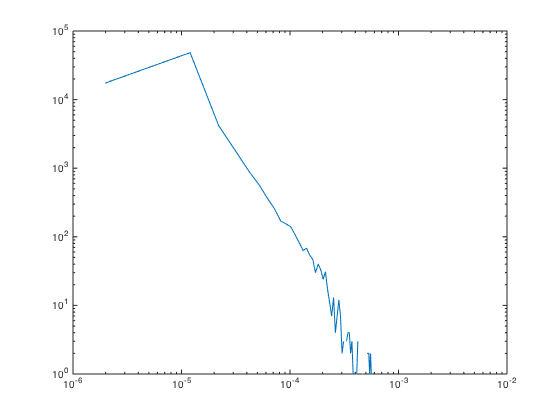
\includegraphics[width=0.3\textwidth]{FIG/10pagerank.png} &
     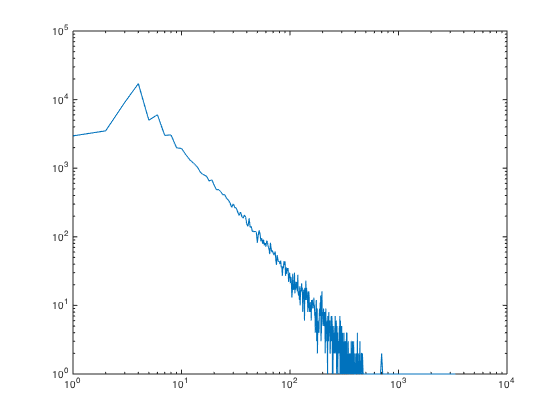
\includegraphics[width=0.3\textwidth]{FIG/10degreedist.png} \\
\end{tabular}
\caption{Result on PageRank Algorithm and Degree Distribution}
\end{center}
\end{figure}

We also did more comprehensive experiments on the 20 datasets to test the functionality of algorithms in the framework and the K-core algorithm we implemented.
Different datasets show different properties when graph mining algorithms are performed on them. We used K = 5 in the experiment as stated in the requirement of the project.

We can find in the table below that some datasets such as \textbf{as-Caida, Cit-HepPh, ca-AstroPh, cit-HepTh, soc-digg, soc-hamsterster, soc-Slashdot0811, text-spanishbook} have relatively big number of nodes but only one or a few connected components. Other datasets such as \textbf{as-skitter, com-amazon, com-dblp, email-Enron} have big number of nodes and relatively big number of connected components. One anomaly type is \textbf{soc-pokec, soc-flickr} in which both number of nodes and number of connected components equal 0. That suggests that no nodes have 5 cores requirement in the dataset. And the small number of connected components suggests that most of the nodes are connected in the graph, only very small number of clusters are formed. The explanation of the formation of connected components is that citations or user relationship form certain groups based on some properties such as interests, regions or languanges.
For example, DBLP dataset has 764 connected components which suggest that many research field are relatively independent and do not cite other areas of research much, resulting in multiple connected components formed. Also, the number of nodes of DBLP is relatively large compared to the original number of nodes, whici is , so we find infer that inside a research area, people cite each other frequently, which helps produce a large number of nodes.
For datasets such as \textbf{soc-hamsterster} and \textbf{cit-HepTh} which include citation information in arXiv's High Energy Physics area and friendships between users of the website hamsterster.com, we can find that only one connected components are formed. The reason is that this is a small area of research or common interest and people in this group are well connected and no significant sub-clusters are formed. The large number of nodes compared to the total number of nodes suggest that research work and users in these fields are highly connected and active, or many of the nodes are of high quality.

For datasets such as \textbf{soc-pokec, soc-flickr} and \textbf{p2p-Gnutella} which no or very few connected components are formed and that the number of nodes in the K-core results are small. The explanation for few connected components are similar to the above, which means that relations of points in the dataset are already highly connected and form a group that no further significant sub-clusters form. The small number of nodes means that nodes such as users in digg.com and flickr.com do not have authorities or hubs who have a lot of followers. Instead, users have simple relationship with each other and are generally equal. Then K=5 K-core algorithm will generate very small number of nodes who have the coreness.

\begin{center}
Table of K-core Algorithm Result for 20 Datasets
\begin{tabular}{ |c|c|c| }
 \hline
 Dataset & Number of Nodes & Number of Connected Components \\
  as-Caida & 1436 & 1 \\
  as-skitter & 9090 & 159 \\
  bio-protein & 57 & 1 \\
  ca-AstroPh & 12574 & 8 \\
  cit-Cora & 384 & 13 \\
  cit-HepPh & 8393 & 3 \\
  cit-HepTh & 21768 & 2 \\
  com-amazon & 19029 & 2090 \\
  com-dblp & 23194 & 764 \\
  email-Enron & 21577 & 180 \\
  p2p-Gnutella31 & 88 & 7 \\
  soc-digg & 1066 & 2 \\
  soc-flickr & 0 & 0 \\
  soc-hamsterster & 1103 & 1 \\
  soc-pokec & 0 & 0 \\
  soc-Slashdot0811 & 20577 & 2 \\
  soc-Youtube & 277 & 4 \\
  soft-jdkdependency & 84 & 1 \\
  text-spanishbook & 1350 & 1 \\
 \hline
\end{tabular}
\end{center}


Degree Distribution Experiment
\begin{figure}[H]
\begin{center}
\begin{tabular}{cc}
     % uncomment the next lines, and give the right ps files
     \includegraphics[width=0.95\textwidth]{FIG/degree1.png}
\end{tabular}
\caption{Result on Degree Distribution Experiment on 20 datasets:Degree}
\end{center}
\end{figure}

\begin{figure}[H]
\begin{center}
\begin{tabular}{cc}
     % uncomment the next lines, and give the right ps files
     \includegraphics[width=0.95\textwidth]{FIG/degree2.png}
\end{tabular}
\caption{Result on Degree Distribution Experiment on 20 datasets:Degree}
\end{center}
\end{figure}

\begin{figure}[H]
\begin{center}
\begin{tabular}{cc}
     % uncomment the next lines, and give the right ps files
     \includegraphics[width=0.95\textwidth]{FIG/indegree1.png}
\end{tabular}
\caption{Result on Degree Distribution Experiment on 20 datasets:InDegree}
\end{center}
\end{figure}

\begin{figure}[H]
\begin{center}
\begin{tabular}{cc}
     % uncomment the next lines, and give the right ps files
     \includegraphics[width=0.95\textwidth]{FIG/indegree2.png}
\end{tabular}
\caption{Result on Degree Distribution Experiment on 20 datasets:inDegree}
\end{center}
\end{figure}

\begin{figure}[H]
\begin{center}
\begin{tabular}{cc}
     % uncomment the next lines, and give the right ps files
     \includegraphics[width=0.95\textwidth]{FIG/outdegree1.png}
\end{tabular}
\caption{Result on Degree Distribution Experiment on 20 datasets:outDegree}
\end{center}
\end{figure}

\begin{figure}[H]
\begin{center}
\begin{tabular}{cc}
     % uncomment the next lines, and give the right ps files
     \includegraphics[width=0.95\textwidth]{FIG/outdegree2.png}
\end{tabular}
\caption{Result on Degree Distribution Experiment on 20 datasets:outDegree}
\end{center}
\end{figure}

Most of the graphs follow the power law. But for some of the graphs, we see strange patterns. We discuss these below.
1. Gnutella P2P: The Out-degree distribution is not a power-law pattern and it has sudden jump in the middle of the picture. It means that about 10 machines connects to all of the machines in the p2p cluster. It might be some master file service machines that stores all of the files in the cluster.
2. JDK dependency: The Out-degree distribution is not a power law pattern, and In-degree distribution shows lots of waves at the tail. We inferred that in Java the relationship between classes is not just simple independent as Java has inherit, interface, implementation. For all the classes, the basement class is Object.class. 
3. Flickr Social: From the Out-degree we found about more than 40000 users who has zero out degree, but from In-degree we found that only 1000 users has zero in degree. This shows that in Flickr most users just upload their photos but they don't care others so they don't follow others. And there are some users who follows large amount of users. Most of the users are followed by some maybe administrative account as most of the users have at least one follower.
4. Pokec Social: The same observation with Flickr also takes place on Pokec.
5. Email EuAll: From the in degree we found that there are almost 200000 accounts that receives zero email, which shows a large amount of mistyped, no-existing or spam email addresses.

PageRank Experiment

\begin{figure}[H]
\begin{center}
\begin{tabular}{cc}
     % uncomment the next lines, and give the right ps files
     \includegraphics[width=0.95\textwidth]{FIG/pagerank1.png}
\end{tabular}
\caption{Result on PageRank Experiment on 20 datasets}
\end{center}
\end{figure}

\begin{figure}[H]
\begin{center}
\begin{tabular}{cc}
     % uncomment the next lines, and give the right ps files
     \includegraphics[width=0.95\textwidth]{FIG/pagerank2.png}
\end{tabular}
\caption{Result on PageRank Experiment on 20 datasets}
\end{center}
\end{figure}

We analyzed the pageRank score and the number of nodes with that score.Half of the graphs show the pattern of power-law, but others are not which described as below.
1. Digg Social: There are several small jump in the descending trend.
2. Flickr Social: the points are more scattered and distributed sparse compared with power-law. As we have mentioned above in degree distribution, due to the social relationship that most of the users are not following anyone else. Or those accounts are zombies accounts.
3. Hamsterster Social: The trending is more or less like power-law but it is not a standard one.
4. Pokec Social: Like Flicker, the points are more scattered. due to the social relationship that most of the users are not following anyone else. Or those accounts are zombies accounts.
5. Youtube Social: After a few ascending, it follows the power-law. We inferred that the reason is most of the Youtebe users using Google account to log in and do the social work. As not all of the google account are active users, there are small amount of very inactive user account which combines the start of the line.
6. Gnutella P2P: As in a P2P network, every node is totally equal to others, there is no way to say which one is more important or not. But there are pagerank difference is just because maybe some of the users has more files than others, but if they are normal users, no one has extraordinary numbers of files unless it has some purpose.
7. JDK dependency: As described in degree distribution, JDK classes has its internal dependency following Obejct Oriented Language Design.
8. Hepth Citation: There is a small ascending trend and then goes with power-law. 

Connected Component Experiment

\begin{figure}[H]
\begin{center}
\begin{tabular}{cc}
     % uncomment the next lines, and give the right ps files
     \includegraphics[width=0.95\textwidth]{FIG/cc1 2.png}
\end{tabular}
\caption{Result on Connected Component Experiment on 20 datasets}
\end{center}
\end{figure}

\begin{figure}[H]
\begin{center}
\begin{tabular}{cc}
     % uncomment the next lines, and give the right ps files
     \includegraphics[width=0.95\textwidth]{FIG/cc2 2.png}
\end{tabular}
\caption{Result on Connected Component Experiment on 20 datasets}
\end{center}
\end{figure}

We analyze the component size and the number of components. We can observe a power relation for components if there are hundreds of components. In all the graphs, we see that either the graph is fully connected, or it has too little number of components or it follows the power-law.
1. Fully connected graph: 
JDK dependency is fully connected because it needs to follow JAVA rules.
Spanish Text is fully connected because it is a graph from words of a book. And words in the book are continuous, which means that all the words are of course in the place one by one and must be fully connected.
Caida AS is fully connected because all the ISP must be connected to the internet network, and make sure all their customers can reach out to where ever they want in the universe, so of course they are fully connected.
2. Few Components:
If a graph shows there are few components, it shows that there are strong connection relationship between nodes. Like in Digg, Hamsterster, Pokec, their users are strongly connected to each other. And for Gnutalla P2P, the number of components is just 12. In protein biology graph, it shows that the protein structure is complicated as they highly connect to each other. And in Hepph and HepTh citation, as they are focusing on papers on High Energy Physics which is really high technical, there are not so many papers like some other fields, so the paper citation is limited.


Eigenvalues Experiment

\begin{figure}[H]
\begin{center}
\begin{tabular}{cc}
     % uncomment the next lines, and give the right ps files
     \includegraphics[width=0.95\textwidth]{FIG/eigenv1.png}
\end{tabular}
\caption{Result on Eigenvalue Experiment on 20 datasets}
\end{center}
\end{figure}

\begin{figure}[H]
\begin{center}
\begin{tabular}{cc}
     % uncomment the next lines, and give the right ps files
     \includegraphics[width=0.95\textwidth]{FIG/eigenv1.png}
\end{tabular}
\caption{Result on Eigenvalue Experiment on 20 datasets}
\end{center}
\end{figure}

We performed eigenvalue calculation on the adjacency matrix of undirected graphs as directed graphs' adjacency matrix is not symmetric and eigenvalues of such graphs can be complex numbers. Eigenvalue analysis is fundamental in terms of the spectral properties of graphs. It can also be used to find approximations to graph measures such as triangle counts.  The algorithms implemented in the {\em graphMiner} framework that we used to do the experiments are Lanczos-SO and QR algorithms.

We plotted comparisons of eigen vectors for certain two of top three eigenvalues. Some datasets such as \textbf{soc-Youtube, Euall} show clear "spoke" like features. Datasets such as \textbf{Gnutella31, bio-protein} have no clear "spoke" features. In fact, if we only plot the very top nodes with the largest eigenvalues, the plots will show clearer spokes, for example, if we use top 100 nodes in the datasets with largest eigenvalues. The plots we have used are called EE-plots, showing the values of nodes in the $i_th$ eigenvector vs. in the $j_th$ eigenvector. Notice the clear ‘spokes’ in top eigenvectors signify the existence of a strongly related group of nodes in near-cliques or bi-cliques. 

With the idea of cliques in mind, we can infer in the datasets that datasets with clear spokes suggest that such datasets have clique relationship, where certain nodes in part of the graph are heavily connected to each other and thus form a small sub-group. \textbf{Euall} for example, is the sender and the recipient of the email data from a large European research institution in a period of time. Thus, people of aquaintance will tend to contact each other often, which create cliques.
Similar cliques occur for \textbf{soc-Youtube} which contain users' friendship. The clique might come from people like the same channel or have similar subscriptions.

Other datasets do not show "spokes" as clear as the above datasets, but that might come from too many nodes are included. If we only plot part of the nodes in the dataset, we might find clearer spokes. Also, in such datasets for example \textbf{bio-protein, Hepth Citation}, we can still find that points in the EE-graph form a cluster instead of randomly distribute. Thus we can infer that there are still cliques in the data, but they are loosely close, that is, nodes in cliques also connect to other nodes that are not apparently similar to nodes in the clique.

Triangle Count Experiment

\begin{figure}[H]
\begin{center}
\begin{tabular}{cc}
     % uncomment the next lines, and give the right ps files
     \includegraphics[width=0.9\textwidth]{FIG/trianglecount.png}
\end{tabular}
\caption{Result on Eigenvalue Experiment on 20 datasets}
\end{center}
\end{figure}

Triangle(three nodes connected to each other) count can answer questions about the community structure of graphs such as if nodes form starts or cliques. In the framework, approximation of triangle counts with high accuracy is done through its connection to eigenvalues. The total number of triangles in a graph is related to the sum of cubes of eigenvalues, and the first few eigenvalues provide extremely good approximations. A slightly more elaborate analysis approximates the number of triangles in which a node participates, using the cubes of the first few eigenvalues and the corresponding eigenvectors.

We can find in the graph that \textbf{Euron Email Communication} have the largest number of triangles and that \textbf{pokec-soc} have the smallest number of triangles. The email data contain emails of an organization for a period of time which apparently point to each other and explains why triangles form very often. In datasets where number of triangles are small, such as \textbf{pokec-soc}, that is because users friendship in this dataset seldom form triangles as the friendship is directed, which reduces the chance of forming a triangle.



